% =====================================================================================
% Clinical TabReD -- CSCI 447 Final Project Report (Project ID P034)
% Built on the course IEEE template (ieeecolor.cls + generic.sty, unchanged).
% Compile:  pdflatex main && bibtex main && pdflatex main && pdflatex main
%           (or upload this folder to Overleaf; compiler pdfLaTeX)
% Numbers: results_summary/, results_{nhanes,brfss,natality}/, for_presentation/tables/.
% =====================================================================================
\documentclass[journal,twoside,web]{ieeecolor}
\usepackage{generic}
\usepackage{cite}
\usepackage{amsmath,amssymb,amsfonts}
\usepackage{graphicx}
\usepackage{algorithm,algorithmic}
\usepackage{booktabs}
\usepackage{multirow}
\usepackage{array}
\usepackage{xcolor}
\usepackage{hyperref}
\hypersetup{hidelinks=true}
\usepackage{textcomp}
\graphicspath{{figures/}}

\def\journalname{CSCI 447 MACHINE LEARNING: THEORY AND PRACTICE, FINAL PROJECT REPORT}
\markboth{\hskip25pc CSCI 447 FINAL PROJECT REPORT, PROJECT ID P034}
{Baktygali and Rakhimzhanov: Clinical TabReD}

% ---- captions: 10 pt Times (course requirement); class default is 8 pt sans --------
\makeatletter
\long\def\@makecaption#1#2{%
  \fontfamily{ptm}\fontseries{m}\fontshape{n}\fontsize{10}{12}\selectfont
  \ifx\@captype\@IEEEtablestring
    \@IEEEtablecaptionsabspace
    \begin{center}{#1}\\ {#2}\end{center}%
    \@IEEEtablecaptionsbespace
  \else
    \@IEEEfigurecaptionsepspace
    \setbox\@tempboxa\hbox{#1.~~#2}%
    \ifdim\wd\@tempboxa>\hsize
      \parbox[t]{\hsize}{\noindent #1.~~#2}%
    \else
      \hbox to\hsize{\box\@tempboxa\hfil}%
    \fi
  \fi}
\def\fnum@figure{Fig.~\thefigure}
\def\fnum@table{TABLE~\thetable}
\makeatother

% ---- float placement ----------------------------------------------------------------
\setcounter{dbltopnumber}{2}
\renewcommand{\dbltopfraction}{0.92}
\renewcommand{\topfraction}{0.92}
\renewcommand{\textfraction}{0.06}
\renewcommand{\floatpagefraction}{0.80}
\renewcommand{\dblfloatpagefraction}{0.80}

% ---- contribution highlighting ------------------------------------------------------
\definecolor{contribframe}{RGB}{31,95,168}
\definecolor{contribbg}{RGB}{234,241,250}
\DeclareRobustCommand{\contrib}[1]{\textbf{\textcolor{contribframe}{[C#1]}}}
\newcommand{\contribbox}[1]{\par\smallskip\noindent
  \fcolorbox{contribframe}{contribbg}{\begin{minipage}{\dimexpr\columnwidth-2\fboxsep-2\fboxrule\relax}#1\end{minipage}}%
  \par\smallskip}
\newcommand{\Dgap}{\ensuremath{\Delta}}

\begin{document}
\title{Clinical TabReD: Evaluating Tabular Machine Learning Models under Temporal Distribution Shift in Healthcare Data}
\author{Nurbek Baktygali (202127847) and Yelzhan Rakhimzhanov (202197093)
\thanks{Final project report for CSCI 447 Machine Learning: Theory and Practice, Fall 2026,
Project ID P034. Instructor: Dr.~Hari Mohan Rai, Department of Computer Science, SCAI,
Nazarbayev University.}
\thanks{The authors are with Nazarbayev University, Astana, Kazakhstan.}}

\maketitle

\begin{abstract}
Clinical models are trained on past patients and used on future ones, but are usually evaluated
with random splits. TabReD showed on industrial data that random splits misjudge performance and
model rankings; it has no healthcare data. We build Clinical TabReD from NHANES 2005--2018 and BRFSS
2017--2023 (diagnosed diabetes) and NCHS natality 2016--2024 (preterm birth), compare five models
on seven TabReD-style splits per dataset with bootstrap confidence intervals and 5-fold
cross-validation, and link each drift to a documented clinical cause. Gradient-boosted trees are
best everywhere (test ROC-AUC 0.900, 0.826, 0.750). Random splits overestimate future performance
on both diabetes datasets and reorder models in NHANES, but not for preterm birth, where a new
same-period comparison shows that later years are simply easier. The type of drift (label shift,
coding revisions) matters more than its size.
\end{abstract}

\begin{IEEEkeywords}
Dataset shift, gradient boosting, healthcare, model evaluation, tabular benchmarks, temporal validation.
\end{IEEEkeywords}

% =====================================================================================
\section{Introduction}
\label{sec:intro}

\IEEEPARstart{C}{linical} models are trained on past patients and applied to future ones, while
laboratories, questionnaires, policies and disease prevalence change in between
\cite{finlayson2021clinician,davis2017calibration}. Random train/test splits ignore this. TabReD
\cite{rubachev2025tabred} showed on eight industrial datasets that time-based splits change both
performance estimates and model rankings, but it contains no healthcare data. We ask whether its
conclusions hold on clinical data:
\begin{itemize}
\item \textbf{RQ1:} Do random splits misjudge future performance and model ranking?
\item \textbf{RQ2:} Which models transfer best to later periods?
\item \textbf{RQ3:} What drifts, and what is its clinical cause?
\item \textbf{RQ4:} Does the type or the size of drift explain the performance gaps?
\end{itemize}

\contribbox{\textbf{\textcolor{contribframe}{Our contributions.}}
\begin{list}{}{\setlength{\leftmargin}{2.5em}\setlength{\labelwidth}{2.2em}%
  \setlength{\labelsep}{0.3em}\setlength{\itemsep}{2pt}\setlength{\topsep}{3pt}%
  \setlength{\parsep}{0pt}\setlength{\itemindent}{0pt}}
\item[\contrib{1}] \textbf{Clinical TabReD:} three leakage-audited public clinical tables (7--9
periods each) with TabReD's split design.
\item[\contrib{2}] \textbf{Drift linked to documented causes:} lab analyzer changes, the Affordable
Care Act, questionnaire revisions, a state reporting law, COVID-19 policies.
\item[\contrib{3}] \textbf{Same-period random-vs-time comparison:} separates ``unseen period'' from
``easier period''; it reverses the preterm-birth conclusion.
\item[\contrib{4}] \textbf{TabReD's claims re-tested on clinical data:} GBDTs stay best, but
XGBoost's lead over the MLP \emph{grows} under time splits in NHANES.
\item[\contrib{5}] \textbf{Reproducible pipeline and notebook} (CSCI447P034.ipynb).
\end{list}}

Fig.~\ref{fig:timeline} shows the project timeline.

\begin{figure*}[!t]
\centering
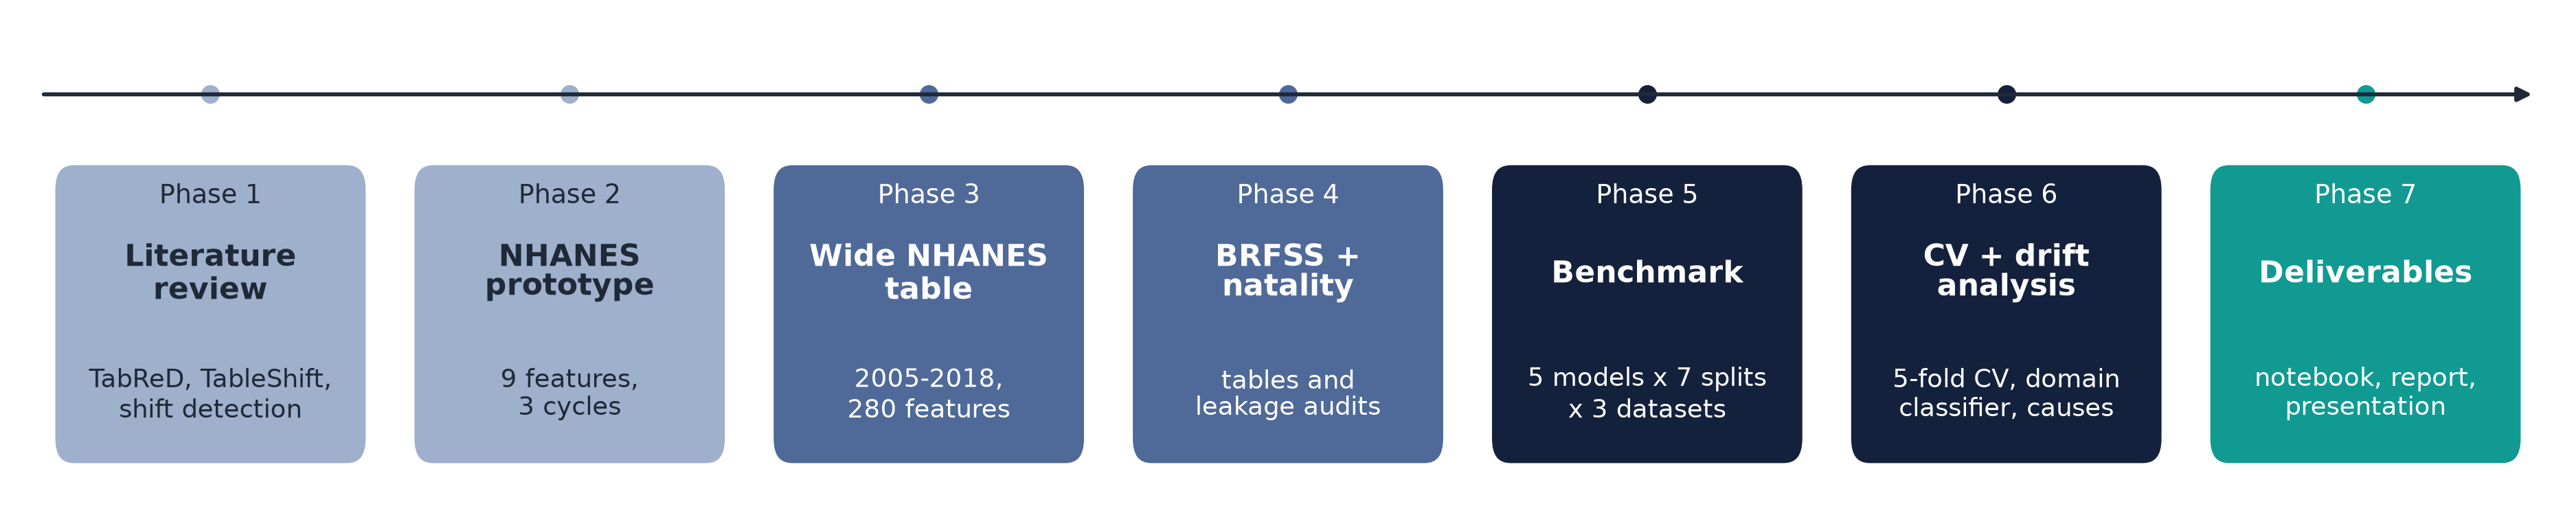
\includegraphics[width=\textwidth]{fig00_timeline.png}
\caption{Project timeline, from the 9-feature NHANES prototype to the three-dataset benchmark,
drift analysis and deliverables.}
\label{fig:timeline}
\end{figure*}

% =====================================================================================
\section{Background and Related Work}
\label{sec:related}
Dataset shift changes $p(\mathbf{x},y)$ between training and deployment \cite{moreno2012unifying}:
covariate shift changes $p(\mathbf{x})$, label shift $p(y)$ \cite{lipton2018detecting}. Temporal
shift degrades clinical models \cite{davis2017calibration,guo2022evaluation}, but studies use
private data and rarely name a cause. TabReD \cite{rubachev2025tabred,tabredrepo} evaluates 18
tabular methods under time splits; TableShift \cite{gardner2023tableshift} includes BRFSS diabetes
but shifts by population group. Tree ensembles still beat deep models on medium-sized tabular data
\cite{grinsztajn2022why}; strong deep baselines are FT-Transformer \cite{gorishniy2021revisiting}
and MLP-PLR \cite{gorishniy2022embeddings}. Domain classifiers characterise shift well
\cite{rabanser2019failing}. Table~\ref{tab:related} shows the gap we address.

\begin{table}[!t]
\caption{Related work and the gap addressed.}
\label{tab:related}
\centering
\setlength{\tabcolsep}{3pt}
\begin{tabular}{@{}p{2.05cm}p{1.6cm}p{1.35cm}p{1.1cm}p{1.1cm}@{}}
\toprule
Work & Data & Shift & Clinical & Cause linked \\
\midrule
TabReD \cite{rubachev2025tabred} & 8 industrial & time & no & no \\
TableShift \cite{gardner2023tableshift} & 15 tasks incl.\ BRFSS & population group & partly & no \\
Grinsztajn \emph{et al.} \cite{grinsztajn2022why} & 45 datasets & none & no & -- \\
Rabanser \emph{et al.} \cite{rabanser2019failing} & simulated & simulated & no & -- \\
Guo \emph{et al.} \cite{guo2022evaluation} & EHR (private) & time & yes & no \\
\midrule
\textbf{This work} & \textbf{NHANES, BRFSS, natality} & \textbf{time} & \textbf{yes} & \textbf{yes} \\
\bottomrule
\end{tabular}
\end{table}

% =====================================================================================
\section{Methodology / Project Approach}
\label{sec:method}
Fig.~\ref{fig:method} shows the workflow. Test periods are used once; preprocessing, model
selection and thresholds use only training and validation periods.

\begin{figure*}[!t]
\centering
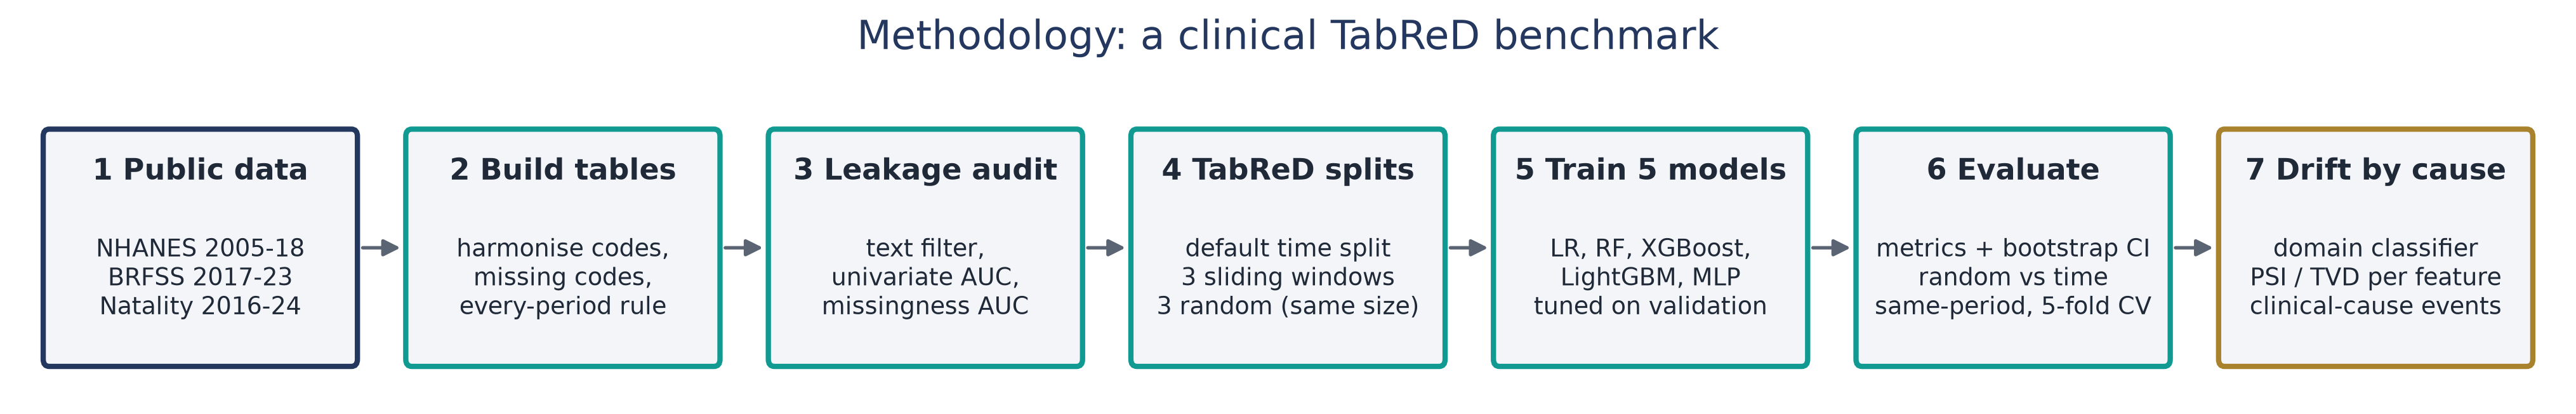
\includegraphics[width=\textwidth]{d01_methodology.png}
\caption{Proposed methodology: data, table construction, leakage audit, TabReD splits, five
models, evaluation, and drift analysis with clinical causes.}
\label{fig:method}
\end{figure*}

\subsection{Data and Leakage Control}
\label{sec:data}
Table~\ref{tab:datasets} lists the datasets \cite{nhanes,brfss,natality}; BRFSS and natality are
sampled to 50,000 rows per year. Special codes become missing, renamed questions are harmonised,
and only features present in every period are kept; IDs, weights, dates and $>$95\%-empty columns
are dropped. Leaking features (diabetes-only questions, consequences of diagnosis, anything
recorded at or after delivery) are removed; afterwards no feature or missingness pattern alone
reaches ROC-AUC 0.80 \contrib{1}.

\begin{table*}[!t]
\caption{The three datasets.}
\label{tab:datasets}
\centering
\resizebox{\textwidth}{!}{%
\begin{tabular}{@{}llllcl@{}}
\toprule
Dataset & Source & Target & Periods & Rows $\times$ features (num./cat.) & Positive rate (first $\rightarrow$ last) \\
\midrule
NHANES 2005--2018 & interview + exam + lab & diagnosed diabetes & 7 two-year cycles & 37,287 $\times$ 280 (102 / 178) & 13.3\% (10.4\% $\rightarrow$ 16.4\%) \\
BRFSS 2017--2023 & telephone survey & diagnosed diabetes & 7 years & 350,000 $\times$ 93 (19 / 74) & 13.6\% (13.7\% $\rightarrow$ 13.9\%) \\
Natality 2016--2024 & birth certificate & preterm birth ($<$37 weeks) & 9 years & 450,000 $\times$ 73 (16 / 57) & 10.2\% (9.6\% $\rightarrow$ 10.5\%) \\
\bottomrule
\end{tabular}}
\end{table*}

\subsection{Split Design}
\label{sec:splits}
Following TabReD (Fig.~\ref{fig:splits}, Table~\ref{tab:splits}):
\begin{itemize}
\item \textbf{Default time split:} train on early periods, validate on the next, test on the
latest. Development/test is 72/28, 71/29 and 78/22, i.e.\ a 70/30--80/20 split ordered in time.
\item \textbf{Sliding windows $k=0,1,2$:} train 3 periods, validate 1, test 1.
\item \textbf{Random splits $k=0,1,2$:} window $k$'s rows shuffled into the same sizes.
\end{itemize}

\begin{figure*}[!t]
\centering
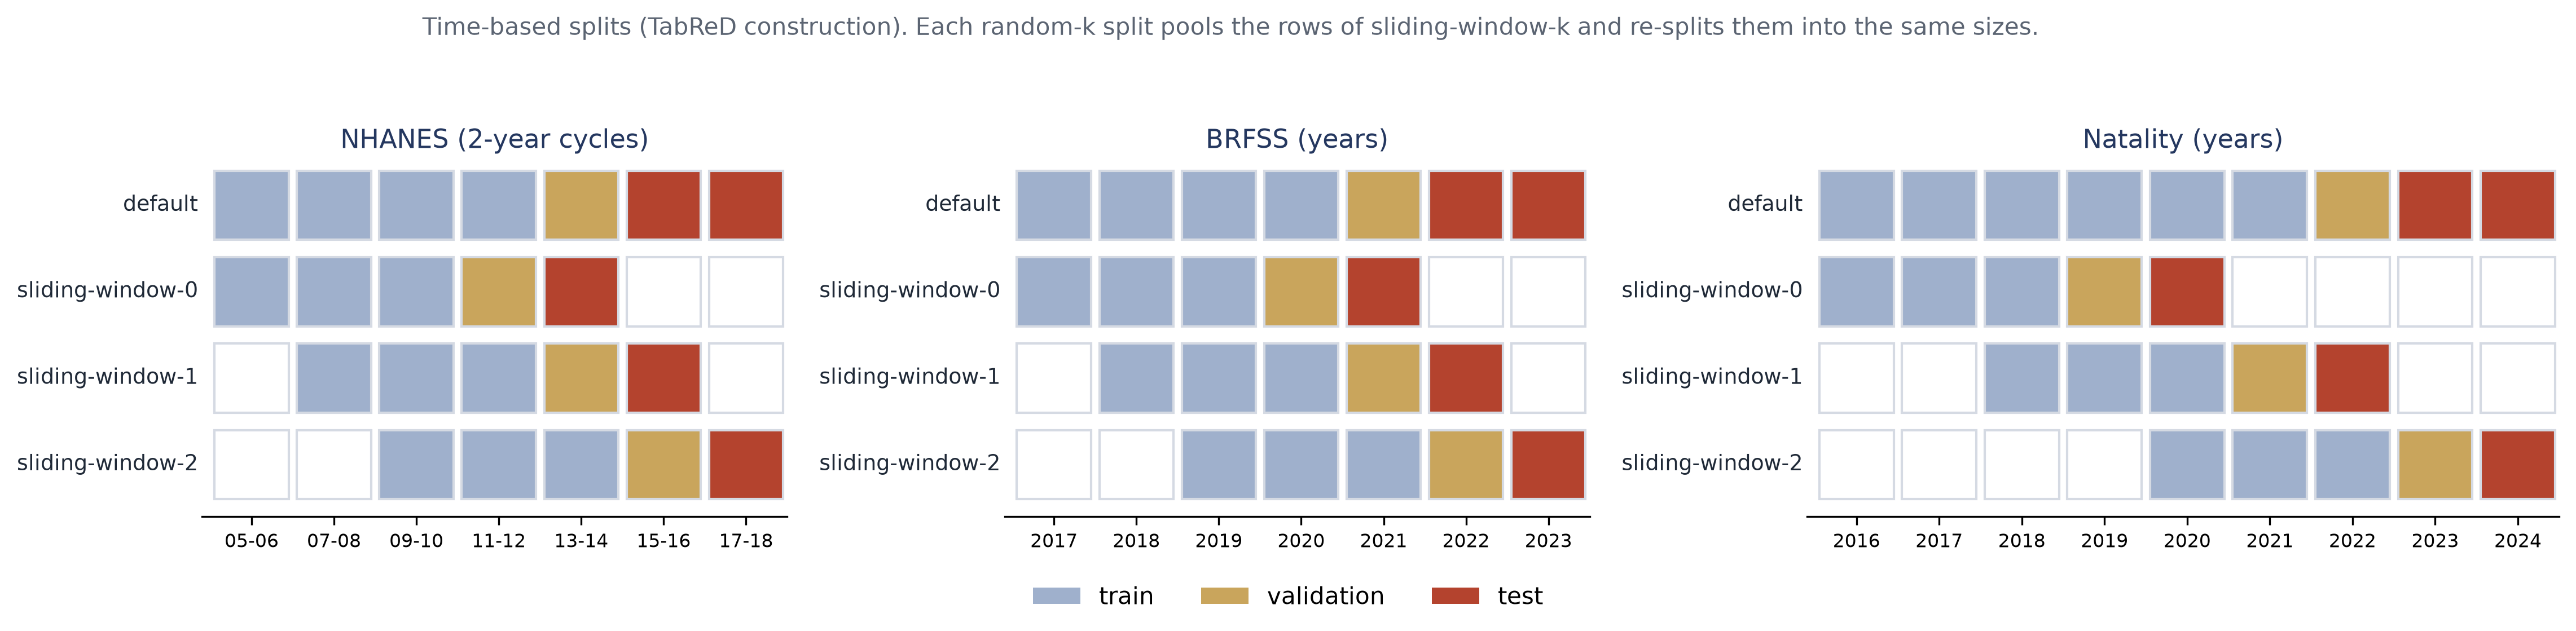
\includegraphics[width=\textwidth]{d03_splits.png}
\caption{Time-based splits per dataset (default and three sliding windows). Random-$k$ re-splits
the rows of window $k$ at random into the same sizes.}
\label{fig:splits}
\end{figure*}

\begin{table*}[!t]
\caption{Default split periods and sizes.}
\label{tab:splits}
\centering
\resizebox{\textwidth}{!}{%
\begin{tabular}{@{}llllll@{}}
\toprule
Dataset & Train (rows, \%) & Validation & Test & Dev./test & Sliding-window test periods \\
\midrule
NHANES & 2005-06 .. 2011-12 (21,427; 57.5\%) & 2013-14 (5,416; 14.5\%) & 2015-16 .. 2017-18 (10,444; 28.0\%) & 72/28 & 2013-14, 2015-16, 2017-18 \\
BRFSS & 2017 .. 2020 (200,000; 57.1\%) & 2021 (50,000; 14.3\%) & 2022 .. 2023 (100,000; 28.6\%) & 71/29 & 2021, 2022, 2023 \\
Natality & 2016 .. 2021 (300,000; 66.7\%) & 2022 (50,000; 11.1\%) & 2023 .. 2024 (100,000; 22.2\%) & 78/22 & 2020, 2022, 2024 \\
\bottomrule
\end{tabular}}
\end{table*}

\subsection{Models}
All models output $\hat p=\hat p(y=1\mid\mathbf{x})$. Logistic regression (LR):
\begin{equation}
\hat p=\sigma(\mathbf{w}^\top\mathbf{x}+b)=1/\bigl(1+e^{-(\mathbf{w}^\top\mathbf{x}+b)}\bigr).
\label{eq:logistic}
\end{equation}
Training minimises the class-balanced log loss
\begin{equation}
\mathcal{L}=-\tfrac{1}{\sum_i\omega_i}\textstyle\sum_i\omega_i\bigl[y_i\ln\hat p_i+(1-y_i)\ln(1-\hat p_i)\bigr],\quad
\omega_i=\tfrac{n}{2n_{y_i}}.
\label{eq:loss}
\end{equation}
Random forest (RF) \cite{breiman2001random} averages bootstrapped trees. XGBoost
\cite{chen2016xgboost} and LightGBM \cite{ke2017lightgbm} fit additive trees:
\begin{equation}
F_M(\mathbf{x})=\textstyle\sum_{m=1}^{M}\eta f_m(\mathbf{x}),\quad
\mathcal{O}=\sum_i\ell(y_i,F(\mathbf{x}_i))+\sum_m\bigl(\gamma T_m+\tfrac12\lambda\lVert\mathbf{v}_m\rVert^2\bigr).
\label{eq:gbdt}
\end{equation}
The MLP uses ReLU layers, $\mathbf{h}_1=\mathrm{ReLU}(\mathbf{W}_1\mathbf{x}+\mathbf{b}_1)$,
$\hat p=\sigma(\mathbf{w}^\top\mathbf{h}_L+b)$, trained with Adam and early stopping.

\subsection{Selection, Metrics and Uncertainty}
The configuration with the best validation PR-AUC is selected; the threshold is
$\tau^\ast=\arg\max_\tau F_1(\tau)$ on validation. Metrics:
\begin{equation}
\mathrm{Acc}=\tfrac{TP+TN}{N},\;\; P=\tfrac{TP}{TP+FP},\;\; R=\tfrac{TP}{TP+FN},\;\; F_1=\tfrac{2PR}{P+R},
\label{eq:metrics}
\end{equation}
\begin{equation}
\mathrm{AUC}=\Pr\bigl(s(\mathbf{x}^{+})>s(\mathbf{x}^{-})\bigr).
\label{eq:auc}
\end{equation}
ROC-AUC \cite{hanley1982meaning} is the main metric because it is independent of threshold and
prevalence; PR-AUC is also reported \cite{saito2015precision}. 95\% CIs use $B=1000$ bootstrap
resamples \cite{efron1993bootstrap}, $\mathrm{CI}=[\hat\theta^\ast_{(0.025)},\hat\theta^\ast_{(0.975)}]$,
paired for model differences and unpaired for random vs.\ time.

\subsection{Random-vs-Time Gap and Same-Period Gap}
Following TabReD, for window $k$ and each model's improvement over the MLP:
\begin{equation}
\Dgap_k=\mathrm{AUC}(\text{random-}k)-\mathrm{AUC}(\text{window-}k),
\label{eq:gap}
\end{equation}
\begin{equation}
I_m=\tfrac13\textstyle\sum_k\bigl(\mathrm{AUC}_{m,k}-\mathrm{AUC}_{\mathrm{MLP},k}\bigr)/\mathrm{AUC}_{\mathrm{MLP},k}\times100\%.
\label{eq:improve}
\end{equation}

\contribbox{\textbf{\textcolor{contribframe}{Same-period gap \contrib{3}.}} The random test set mixes
all periods of the window; the time test set is the last period only. We also score random-$k$
only on its rows $\mathcal{T}_k$ from window $k$'s test period:
\begin{equation}
\Dgap^{\mathrm{same}}_k=\mathrm{AUC}(\text{random-}k\text{ on }\mathcal{T}_k)-\mathrm{AUC}(\text{window-}k).
\label{eq:samegap}
\end{equation}}

\subsection{Cross-Validation Strategy}
5-fold stratified CV \cite{kohavi1995study} runs on the development periods (train + validation)
of the default split with the selected hyperparameters, threshold 0.5. We report
$\bar\theta=\frac15\sum_j\theta_j$ and its standard deviation. CV measures in-period performance;
comparing it with the time-split test is another view of random vs.\ time.

\subsection{Drift Measurement}
A domain classifier \cite{rabanser2019failing} (logistic regression, 5-fold CV ROC-AUC) separates
training from test rows; 0.5 means no shift. Per feature we use
\begin{equation}
\mathrm{PSI}=\textstyle\sum_b(q_b-p_b)\ln\frac{q_b}{p_b},\qquad \mathrm{TVD}=\tfrac12\sum_c\lvert p_c-q_c\rvert,
\label{eq:psi}
\end{equation}
over 10 quantile bins (numeric) \cite{siddiqi2006credit} or categories. The largest changes are
matched to CDC/NCHS documentation \cite{nhanesdoc} \contrib{2}. Algorithm~\ref{alg:bench}
summarises the benchmark.

\begin{algorithm}[!t]
\caption{Clinical TabReD benchmark for one dataset.}\label{alg:bench}
\begin{algorithmic}[1]
\REQUIRE table $D$ with periods; grids $G_m$; seed $s$
\ENSURE test metrics with CIs; gaps $\Dgap_k$, $\Dgap^{\mathrm{same}}_k$
\STATE $S\gets\{$default, window-0..2, random-0..2$\}$
\FOR{each split (train, val, test) in $S$}
  \FOR{each model $m$ and configuration $\theta\in G_m$}
    \STATE fit preprocessing + $m_\theta$ on train; score val PR-AUC
  \ENDFOR
  \STATE pick $\theta^\ast$; set $\tau^\ast$ on val; score test once
\ENDFOR
\STATE bootstrap CIs; paired model differences
\STATE $\Dgap_k$ \eqref{eq:gap} and $\Dgap^{\mathrm{same}}_k$ \eqref{eq:samegap}, $k=0,1,2$
\STATE domain classifier; PSI/TVD \eqref{eq:psi}; documented events
\end{algorithmic}
\end{algorithm}

% =====================================================================================
\section{Implementation and System Design}
\label{sec:impl}
Table~\ref{tab:stack} lists the stack \cite{pedregosa2011scikit,hunter2007matplotlib} and
Fig.~\ref{fig:arch} the pipeline: median imputation and scaling for numeric features, mode
imputation and one-hot encoding for categorical ones, fitted on training data only. Imbalance is
handled by balanced class weights (LR, RF), \texttt{scale\_pos\_weight} (GBDTs) and balanced sample
weights (MLP; batch 128, learning rate $10^{-3}$, patience 10). Grids are in Table~\ref{tab:grids}.
The 105 model selections (5 models $\times$ 7 splits $\times$ 3 datasets) take about 3 hours on a
16-core CPU, seed 42. The notebook reproduces the saved results \contrib{5}.

\begin{table}[!t]
\caption{Technology stack.}
\label{tab:stack}
\centering
\begin{tabular}{@{}lll@{}}
\toprule
Component & Version & Role \\
\midrule
Python & 3.12.3 & language \\
numpy / pandas & 2.5.4 / 3.1.1 & data \\
scikit-learn & 1.9.1 & LR, RF, MLP, metrics \\
xgboost & 3.4.1 & XGBoost \\
lightgbm & 4.7.0 & LightGBM \\
matplotlib & 3.11.2 & figures \\
Hardware & 16-core CPU & no GPU \\
\bottomrule
\end{tabular}
\end{table}

\begin{table}[!t]
\caption{Hyperparameter grids.}
\label{tab:grids}
\centering
\resizebox{\columnwidth}{!}{%
\begin{tabular}{@{}ll@{}}
\toprule
Model & Grid \\
\midrule
LR & $C\in\{0.01, 0.1, 1, 10\}$ \\
RF & 300 trees; depth $\in\{6,10,\text{none}\}$; min.\ leaf $\in\{1,10\}$ \\
XGBoost & 300 trees; $\eta\in\{0.03,0.1\}$; depth $\in\{3,5\}$ \\
LightGBM & 300 trees; $\eta\in\{0.03,0.1\}$; leaves $\in\{7,31\}$ \\
MLP & hidden $\in\{(64),(64,32)\}$; $\alpha\in\{10^{-4},10^{-2}\}$ \\
\bottomrule
\end{tabular}}
\end{table}

\begin{figure*}[!t]
\centering
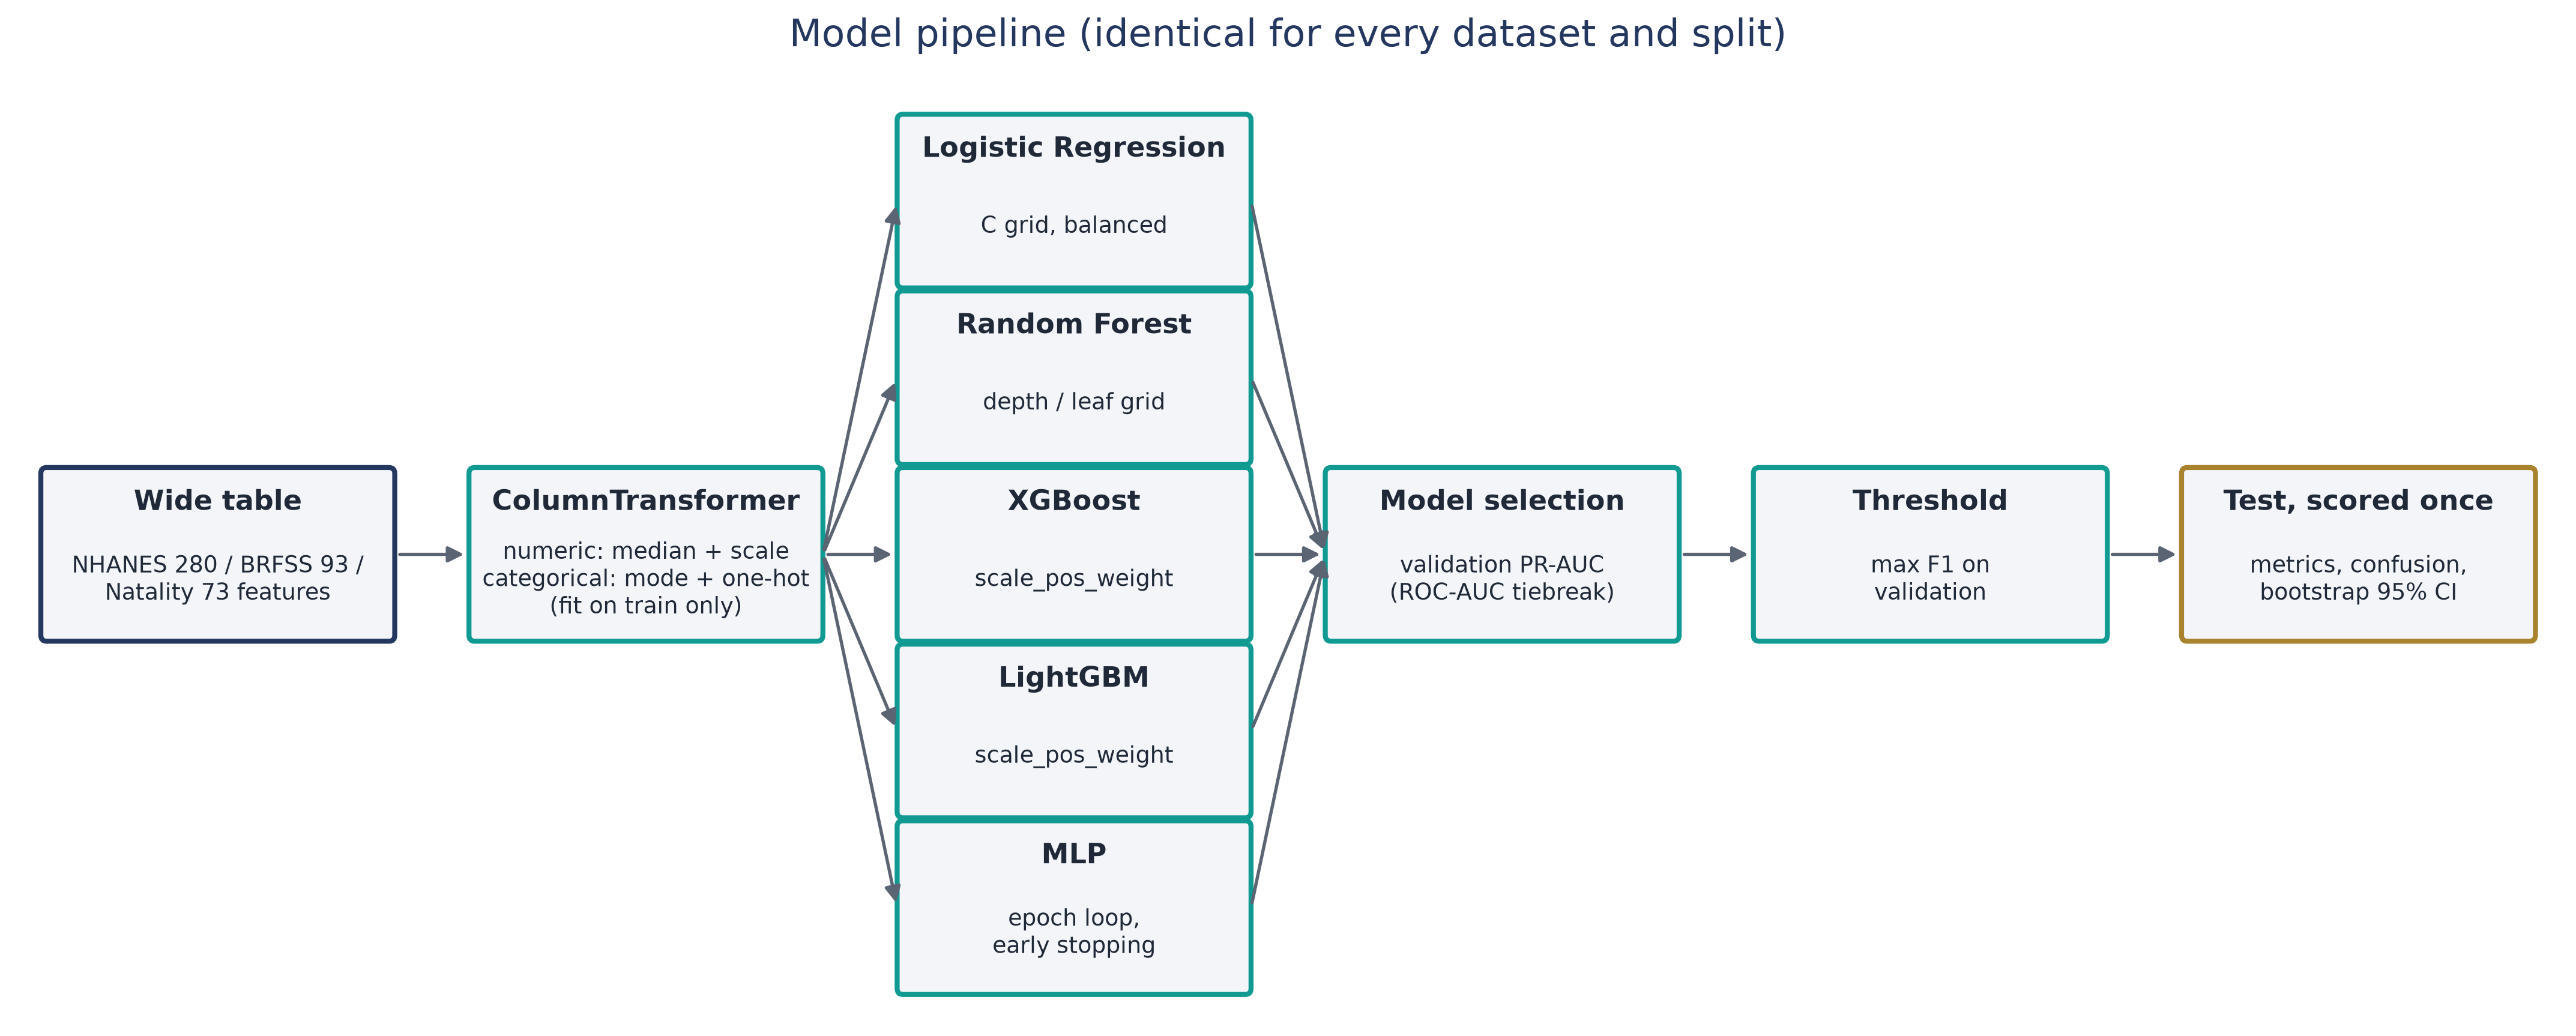
\includegraphics[width=0.86\textwidth]{d02_architecture.png}
\caption{System architecture: preprocessing fitted on training data, five models, selection and
threshold on validation, single test evaluation with bootstrap CIs.}
\label{fig:arch}
\end{figure*}

% =====================================================================================
\section{Evaluation and Results}
\label{sec:results}

\subsection{Default Time Split}
GBDTs are best on all datasets (Table~\ref{tab:default}, Fig.~\ref{fig:auc}). NHANES separates
models most (0.876--0.900); BRFSS and natality differ by about 0.005. In NHANES the
validation-selected MLP is significantly worse on the test years than XGBoost and LightGBM
(Table~\ref{tab:paired}): one validation period does not reliably pick the best future model.

\begin{table*}[!t]
\caption{Test performance on the default time split (threshold $\tau^\ast$ from validation; 95\%
bootstrap CIs). Bold: best ROC-AUC. Sel.: selected on validation.}
\label{tab:default}
\centering
\resizebox{\textwidth}{!}{%
\begin{tabular}{@{}llcccccccc@{}}
\toprule
Dataset & Model & Accuracy & Precision & Recall & $F_1$ & ROC-AUC [95\% CI] & PR-AUC [95\% CI] & $\tau^\ast$ & Sel. \\
\midrule
\multirow{5}{*}{NHANES} & Logistic regression & 0.849 & 0.515 & 0.720 & 0.601 & 0.882 [0.872, 0.891] & 0.619 [0.594, 0.645] & 0.714 & \\
 & Random forest & 0.829 & 0.471 & 0.707 & 0.566 & 0.876 [0.867, 0.884] & 0.571 [0.544, 0.597] & 0.468 & \\
 & XGBoost & 0.868 & 0.571 & 0.659 & 0.612 & \textbf{0.900} [0.892, 0.908] & 0.654 [0.630, 0.677] & 0.727 & \\
 & LightGBM & 0.861 & 0.548 & 0.675 & 0.605 & 0.899 [0.892, 0.906] & 0.646 [0.622, 0.669] & 0.714 & \\
 & MLP & 0.863 & 0.555 & 0.671 & 0.607 & 0.887 [0.878, 0.895] & 0.634 [0.608, 0.661] & 0.718 & yes \\
\midrule
\multirow{5}{*}{BRFSS} & Logistic regression & 0.801 & 0.365 & 0.608 & 0.456 & 0.822 [0.819, 0.825] & 0.409 [0.401, 0.418] & 0.641 & \\
 & Random forest & 0.804 & 0.368 & 0.586 & 0.452 & 0.821 [0.818, 0.825] & 0.409 [0.401, 0.418] & 0.545 & \\
 & XGBoost & 0.811 & 0.377 & 0.582 & 0.458 & 0.824 [0.821, 0.827] & 0.418 [0.410, 0.427] & 0.663 & yes \\
 & LightGBM & 0.814 & 0.383 & 0.573 & 0.459 & \textbf{0.826} [0.823, 0.829] & 0.422 [0.414, 0.431] & 0.682 & \\
 & MLP & 0.808 & 0.375 & 0.588 & 0.458 & 0.824 [0.821, 0.827] & 0.415 [0.406, 0.423] & 0.689 & \\
\midrule
\multirow{5}{*}{Natality} & Logistic regression & 0.883 & 0.422 & 0.340 & 0.376 & 0.744 [0.739, 0.749] & 0.363 [0.353, 0.373] & 0.725 & \\
 & Random forest & 0.869 & 0.370 & 0.381 & 0.376 & 0.744 [0.739, 0.750] & 0.348 [0.339, 0.358] & 0.572 & \\
 & XGBoost & 0.857 & 0.346 & 0.420 & 0.379 & \textbf{0.750} [0.745, 0.756] & 0.369 [0.360, 0.379] & 0.652 & yes \\
 & LightGBM & 0.871 & 0.379 & 0.382 & 0.380 & \textbf{0.750} [0.745, 0.756] & 0.368 [0.358, 0.378] & 0.690 & \\
 & MLP & 0.877 & 0.398 & 0.356 & 0.376 & 0.746 [0.740, 0.751] & 0.364 [0.355, 0.375] & 0.736 & \\
\bottomrule
\end{tabular}}
\end{table*}

\begin{figure*}[!t]
\centering
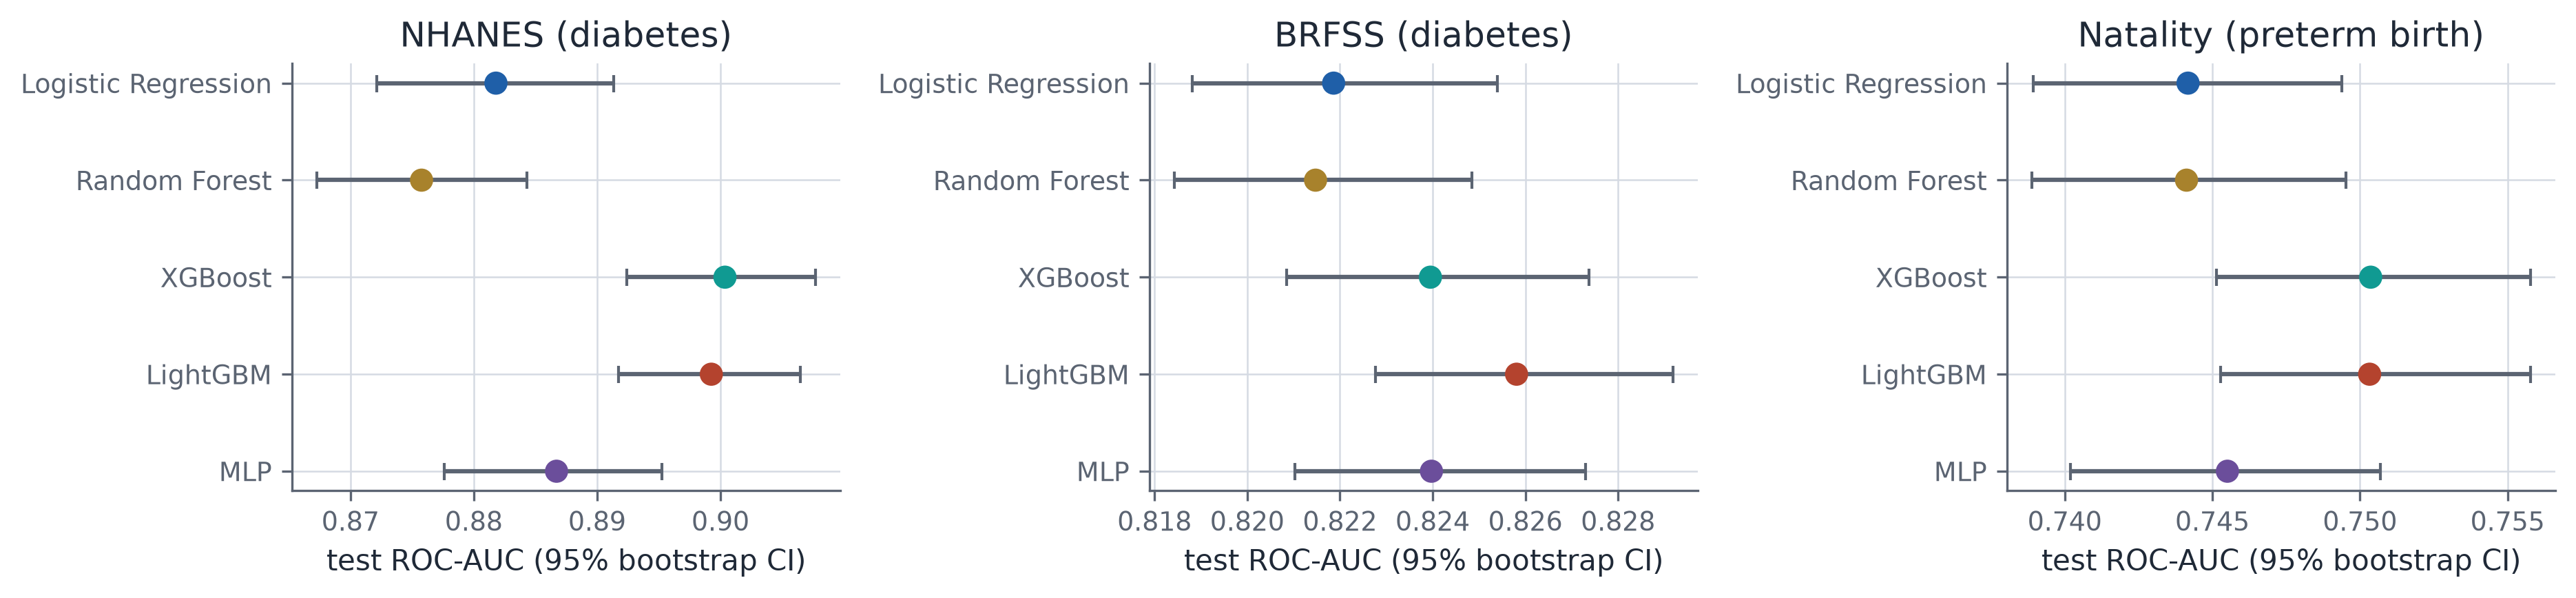
\includegraphics[width=\textwidth]{fig02_default_auc_ci.png}
\caption{Default-split test ROC-AUC per model with 95\% bootstrap CIs.}
\label{fig:auc}
\end{figure*}

\begin{table}[!t]
\caption{Paired bootstrap ROC-AUC difference: validation-selected model minus other model.
$^\ast$: CI excludes zero.}
\label{tab:paired}
\centering
\resizebox{\columnwidth}{!}{%
\begin{tabular}{@{}lll@{}}
\toprule
Dataset (selected) & Other & Difference [95\% CI] \\
\midrule
\multirow{4}{*}{NHANES (MLP)} & XGBoost & $-0.0137$ [$-0.0203$, $-0.0069$]$^\ast$ \\
 & LightGBM & $-0.0125$ [$-0.0193$, $-0.0058$]$^\ast$ \\
 & LR & $+0.0049$ [0.0022, 0.0078]$^\ast$ \\
 & RF & $+0.0109$ [0.0030, 0.0186]$^\ast$ \\
\midrule
\multirow{4}{*}{BRFSS (XGBoost)} & LightGBM & $-0.0019$ [$-0.0026$, $-0.0011$]$^\ast$ \\
 & MLP & $-0.0000$ [$-0.0010$, 0.0010] \\
 & LR & $+0.0021$ [0.0009, 0.0032]$^\ast$ \\
 & RF & $+0.0025$ [0.0014, 0.0036]$^\ast$ \\
\midrule
\multirow{4}{*}{Natality (XGBoost)} & LightGBM & $+0.0000$ [$-0.0008$, 0.0008] \\
 & MLP & $+0.0049$ [0.0031, 0.0067]$^\ast$ \\
 & LR & $+0.0062$ [0.0044, 0.0080]$^\ast$ \\
 & RF & $+0.0062$ [0.0043, 0.0082]$^\ast$ \\
\bottomrule
\end{tabular}}
\end{table}

\subsection{ROC Curves, Confusion Matrices and Training Curves}
ROC curves nearly coincide on BRFSS and natality (Fig.~\ref{fig:roc}). Recall of the selected
model is 0.67 (NHANES), 0.58 (BRFSS) and 0.42 (natality) (Fig.~\ref{fig:cm}). The MLP's validation
loss bottoms out after 3--4 epochs while training loss keeps falling (Fig.~\ref{fig:curves});
early stopping keeps the best epoch.

\begin{figure*}[!t]
\centering
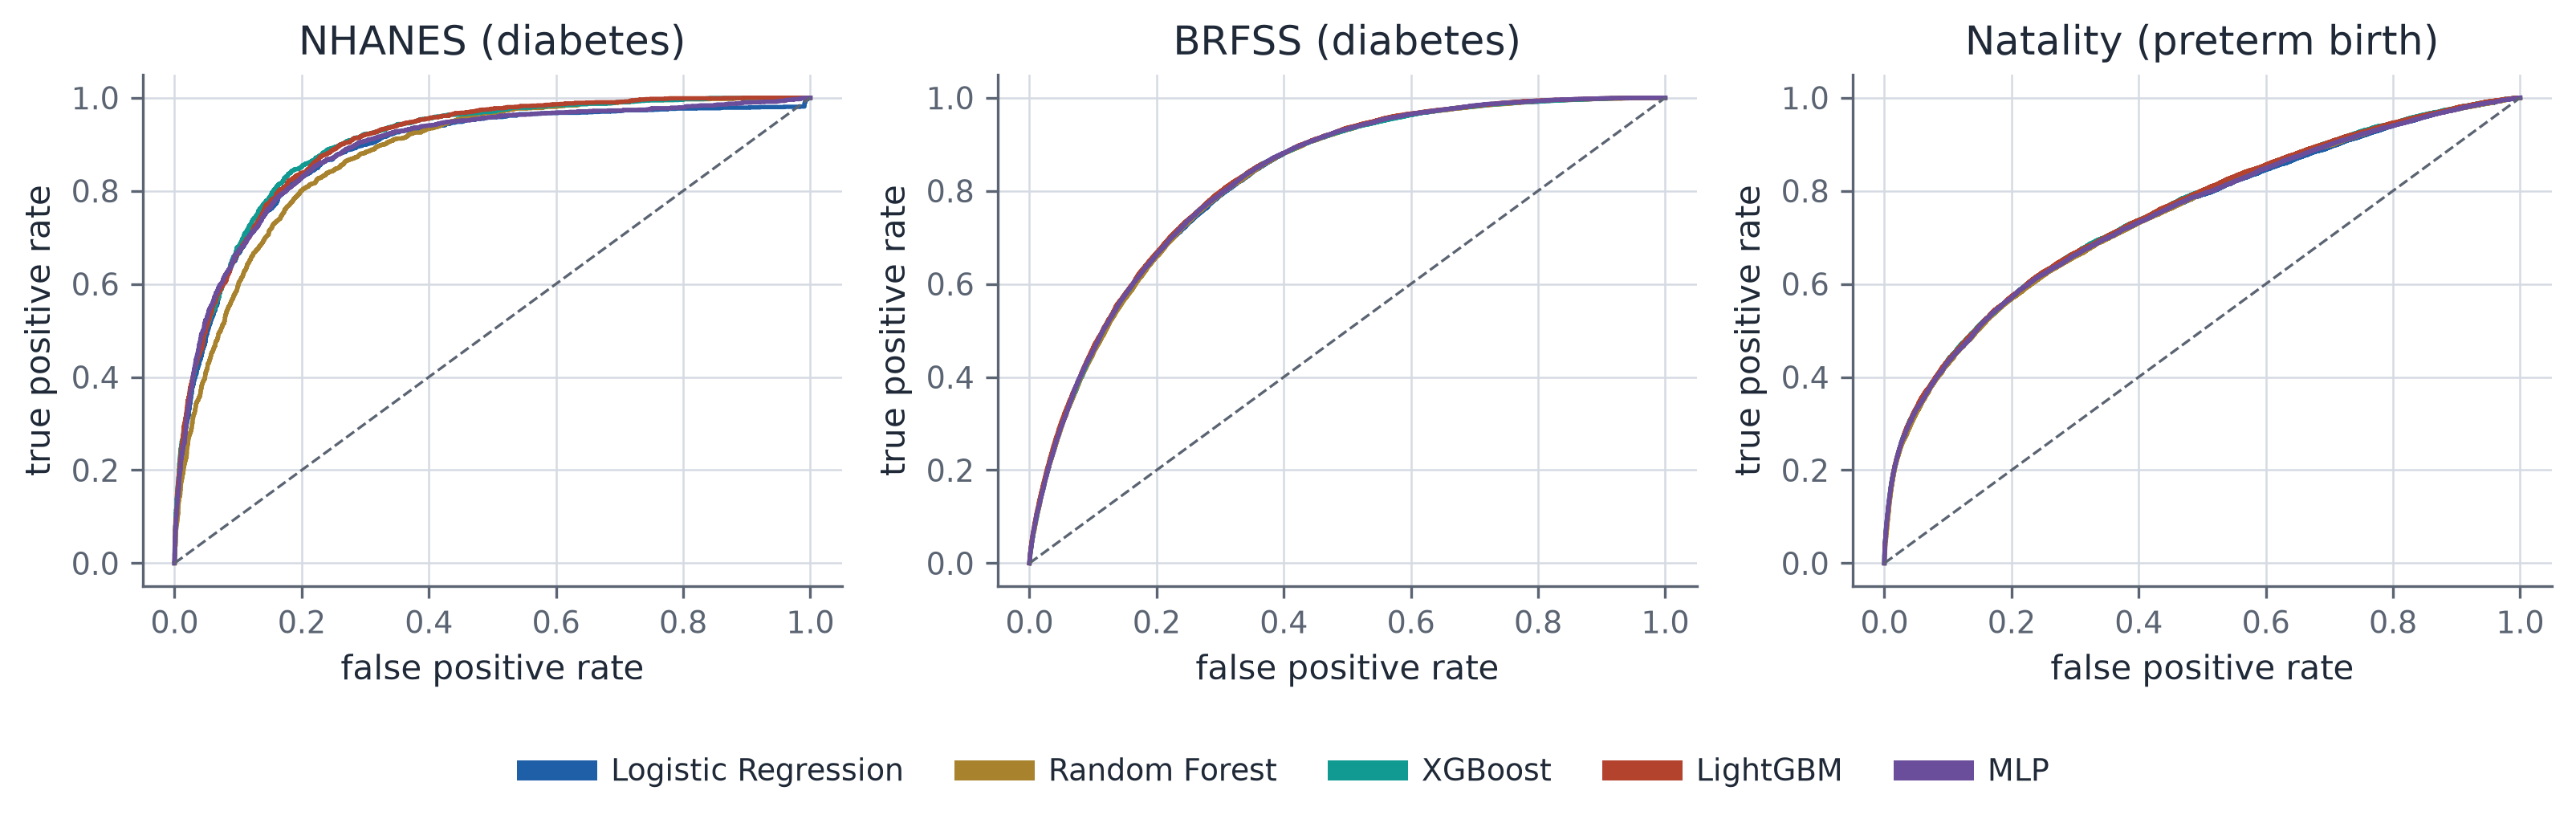
\includegraphics[width=0.92\textwidth]{fig04_roc_curves.png}
\caption{ROC curves on the default test periods.}
\label{fig:roc}
\end{figure*}

\begin{figure*}[!t]
\centering
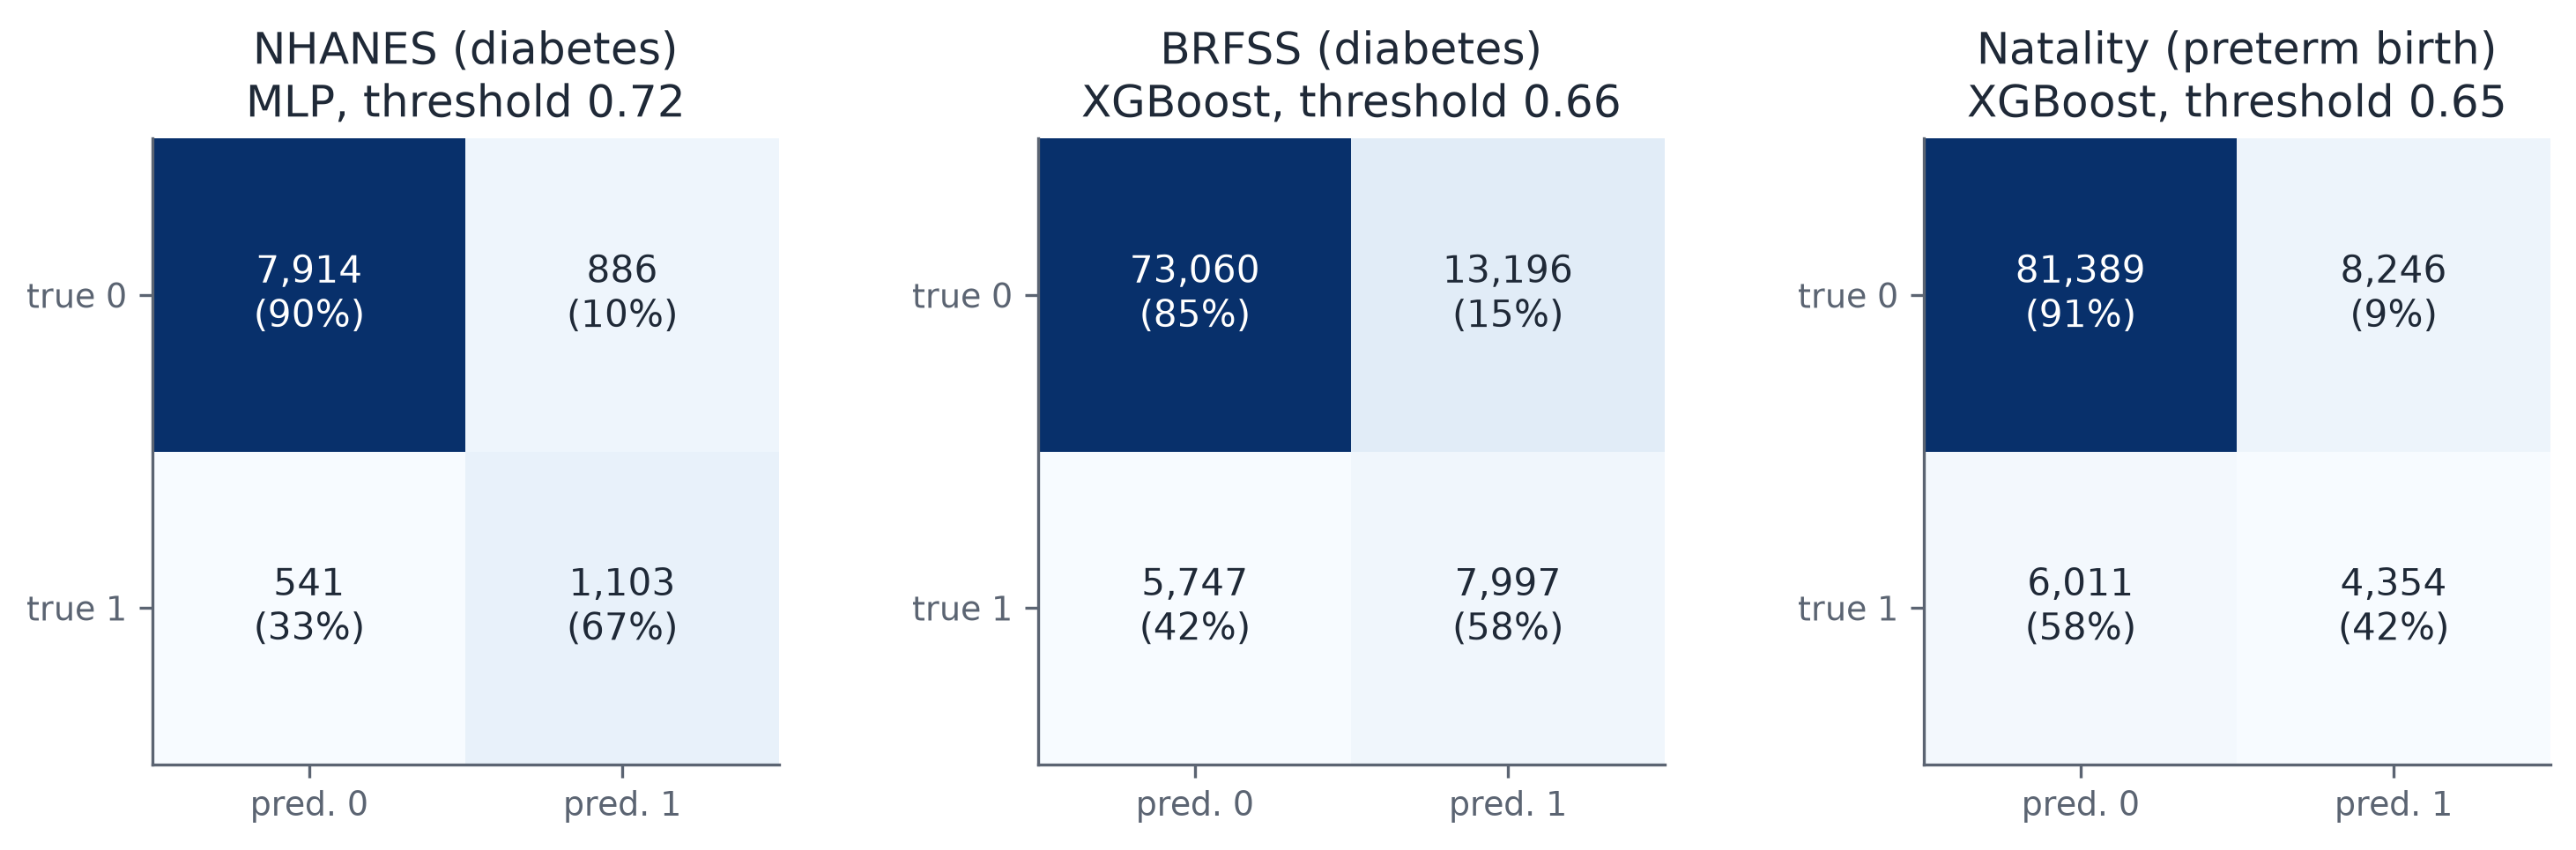
\includegraphics[width=0.86\textwidth]{fig05_confusion_matrices.png}
\caption{Confusion matrices of the validation-selected model (threshold $\tau^\ast$; counts and row
percentages).}
\label{fig:cm}
\end{figure*}

\begin{figure*}[!t]
\centering
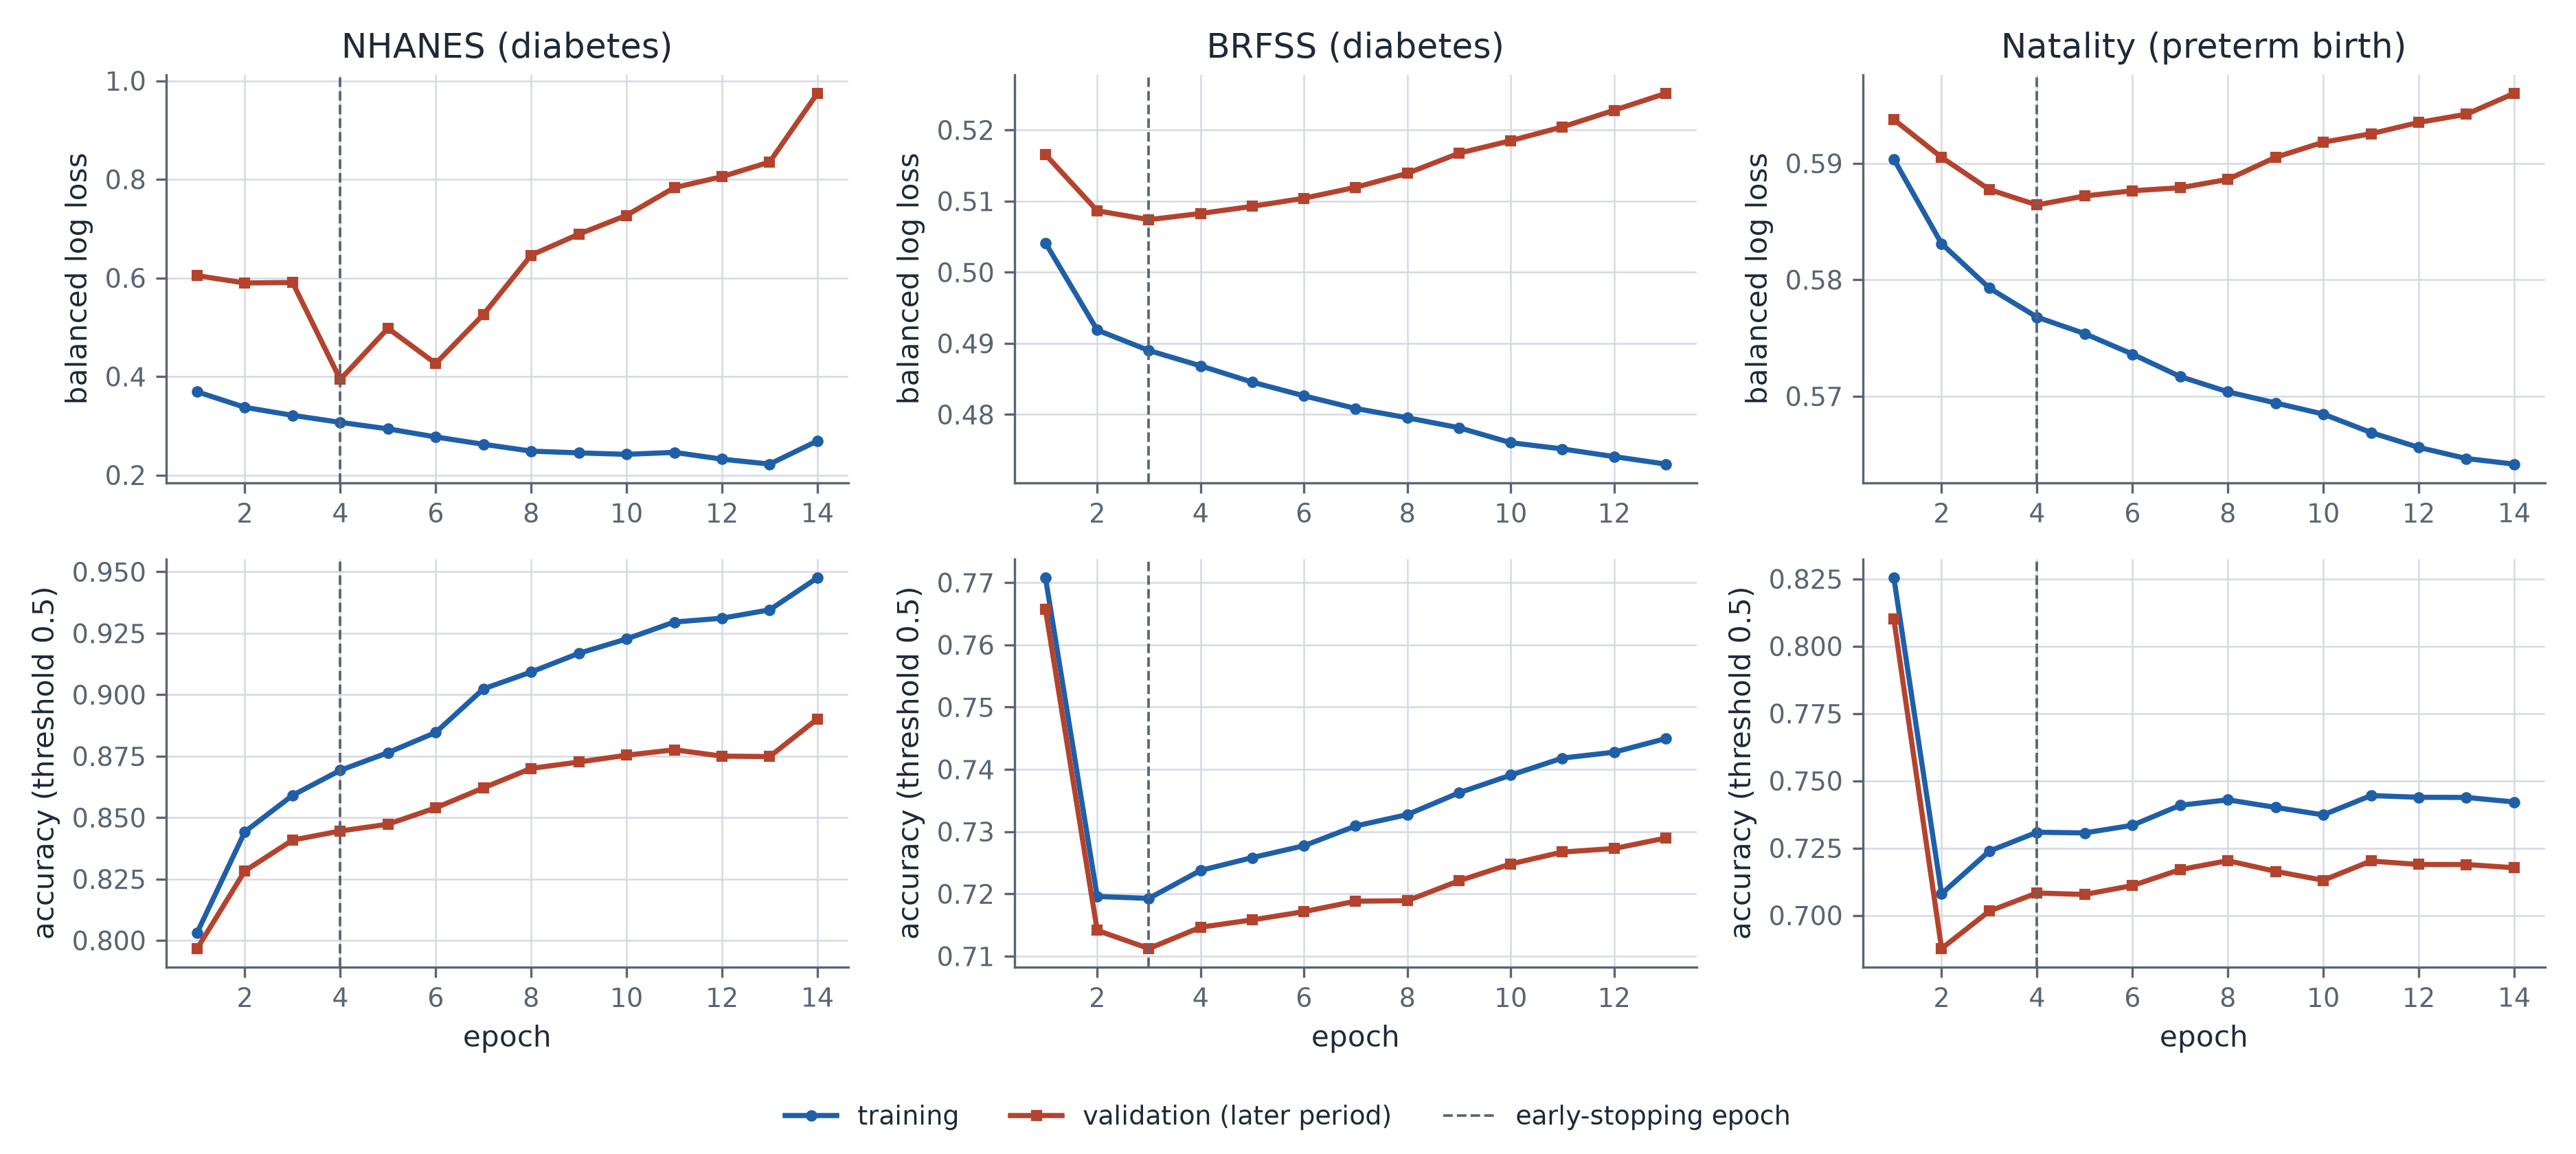
\includegraphics[width=\textwidth]{fig11_mlp_loss_accuracy.png}
\caption{MLP training curves on the default split: loss (top) and accuracy at threshold 0.5
(bottom); validation is a later period. Dashed line: early-stopping epoch.}
\label{fig:curves}
\end{figure*}

\subsection{Cross-Validation}
CV is stable (ROC-AUC std $\le$0.005) and ranks GBDTs first (Table~\ref{tab:cv},
Fig.~\ref{fig:cv}). It exceeds the future test for NHANES (0.91 vs.\ 0.88--0.90) and BRFSS (0.83
vs.\ 0.82--0.83), and matches it for natality (0.75).

\begin{table*}[!t]
\caption{5-fold stratified CV on the development periods (mean $\pm$ std, threshold 0.5).}
\label{tab:cv}
\centering
\resizebox{\textwidth}{!}{%
\begin{tabular}{@{}llcccccc@{}}
\toprule
Dataset & Model & Accuracy & Precision & Recall & $F_1$ & ROC-AUC & PR-AUC \\
\midrule
\multirow{5}{*}{NHANES} & Logistic regression & 0.831 $\pm$ 0.007 & 0.409 $\pm$ 0.011 & 0.835 $\pm$ 0.015 & 0.549 $\pm$ 0.010 & 0.910 $\pm$ 0.005 & 0.612 $\pm$ 0.026 \\
 & Random forest & 0.876 $\pm$ 0.006 & 0.498 $\pm$ 0.019 & 0.619 $\pm$ 0.019 & 0.552 $\pm$ 0.016 & 0.893 $\pm$ 0.005 & 0.564 $\pm$ 0.017 \\
 & XGBoost & 0.852 $\pm$ 0.004 & 0.444 $\pm$ 0.007 & 0.812 $\pm$ 0.017 & 0.574 $\pm$ 0.007 & \textbf{0.914} $\pm$ 0.005 & 0.636 $\pm$ 0.019 \\
 & LightGBM & 0.846 $\pm$ 0.005 & 0.433 $\pm$ 0.009 & 0.800 $\pm$ 0.014 & 0.562 $\pm$ 0.007 & 0.913 $\pm$ 0.005 & 0.632 $\pm$ 0.014 \\
 & MLP & 0.839 $\pm$ 0.018 & 0.423 $\pm$ 0.035 & 0.806 $\pm$ 0.045 & 0.553 $\pm$ 0.020 & 0.908 $\pm$ 0.005 & 0.618 $\pm$ 0.018 \\
\midrule
\multirow{5}{*}{BRFSS} & Logistic regression & 0.731 $\pm$ 0.001 & 0.306 $\pm$ 0.001 & 0.782 $\pm$ 0.005 & 0.440 $\pm$ 0.002 & 0.830 $\pm$ 0.002 & 0.419 $\pm$ 0.004 \\
 & Random forest & 0.788 $\pm$ 0.002 & 0.350 $\pm$ 0.002 & 0.668 $\pm$ 0.005 & 0.460 $\pm$ 0.002 & 0.829 $\pm$ 0.002 & 0.420 $\pm$ 0.002 \\
 & XGBoost & 0.733 $\pm$ 0.002 & 0.308 $\pm$ 0.003 & 0.786 $\pm$ 0.006 & 0.443 $\pm$ 0.003 & 0.833 $\pm$ 0.003 & 0.429 $\pm$ 0.002 \\
 & LightGBM & 0.721 $\pm$ 0.002 & 0.301 $\pm$ 0.002 & 0.805 $\pm$ 0.006 & 0.438 $\pm$ 0.003 & \textbf{0.834} $\pm$ 0.003 & 0.430 $\pm$ 0.001 \\
 & MLP & 0.712 $\pm$ 0.032 & 0.296 $\pm$ 0.018 & 0.810 $\pm$ 0.040 & 0.433 $\pm$ 0.015 & 0.832 $\pm$ 0.003 & 0.425 $\pm$ 0.002 \\
\midrule
\multirow{5}{*}{Natality} & Logistic regression & 0.780 $\pm$ 0.002 & 0.246 $\pm$ 0.002 & 0.565 $\pm$ 0.002 & 0.343 $\pm$ 0.002 & 0.745 $\pm$ 0.003 & 0.365 $\pm$ 0.007 \\
 & Random forest & 0.848 $\pm$ 0.001 & 0.323 $\pm$ 0.003 & 0.454 $\pm$ 0.001 & 0.378 $\pm$ 0.002 & 0.744 $\pm$ 0.003 & 0.349 $\pm$ 0.007 \\
 & XGBoost & 0.786 $\pm$ 0.002 & 0.253 $\pm$ 0.003 & 0.566 $\pm$ 0.004 & 0.349 $\pm$ 0.003 & 0.751 $\pm$ 0.002 & 0.372 $\pm$ 0.007 \\
 & LightGBM & 0.777 $\pm$ 0.003 & 0.246 $\pm$ 0.003 & 0.582 $\pm$ 0.002 & 0.346 $\pm$ 0.002 & \textbf{0.752} $\pm$ 0.002 & 0.372 $\pm$ 0.006 \\
 & MLP & 0.782 $\pm$ 0.029 & 0.250 $\pm$ 0.023 & 0.563 $\pm$ 0.038 & 0.344 $\pm$ 0.015 & 0.745 $\pm$ 0.002 & 0.364 $\pm$ 0.007 \\
\bottomrule
\end{tabular}}
\end{table*}

\begin{figure*}[!t]
\centering
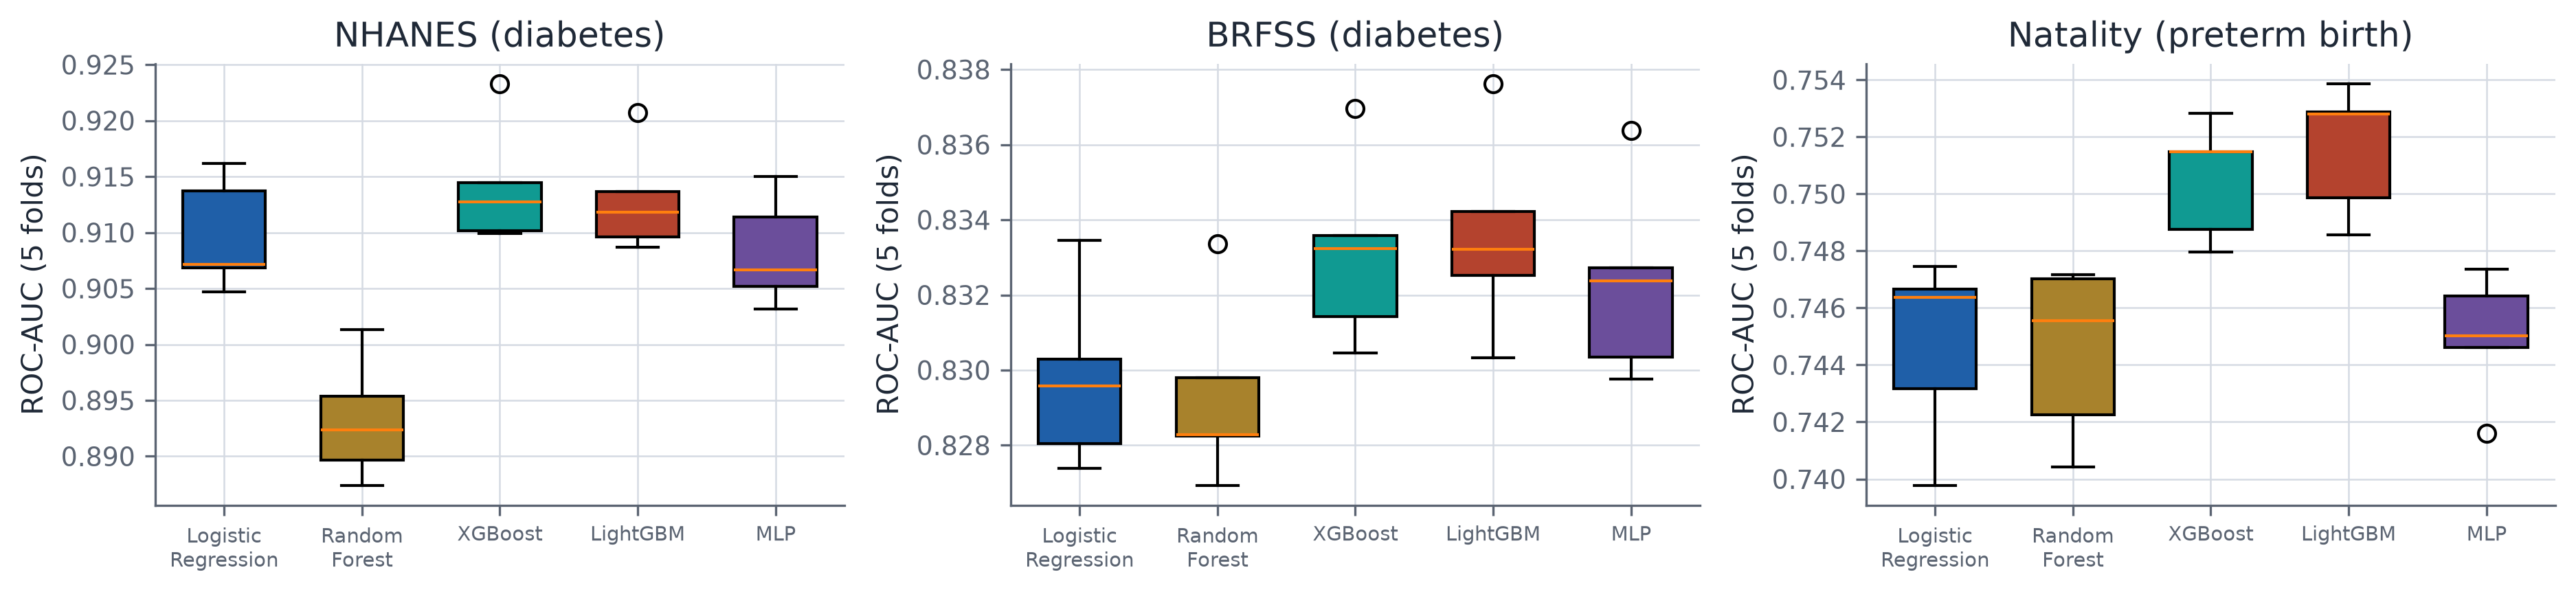
\includegraphics[width=\textwidth]{fig09_cross_validation.png}
\caption{5-fold CV ROC-AUC per fold (dots) and mean (tick).}
\label{fig:cv}
\end{figure*}

\subsection{Random vs.\ Time Splits}
Random splits overestimate future performance on both diabetes datasets (Fig.~\ref{fig:rvt},
Table~\ref{tab:rvt}). BRFSS: $+0.006$ to $+0.007$ for every model, significant in 9 of 15
model-windows. NHANES: up to $+0.02$ in 2015--16, and the MLP drops from 2nd (random) to 4th
(time). Natality shows the opposite ($-0.003$ to $-0.006$).

\begin{figure*}[!t]
\centering
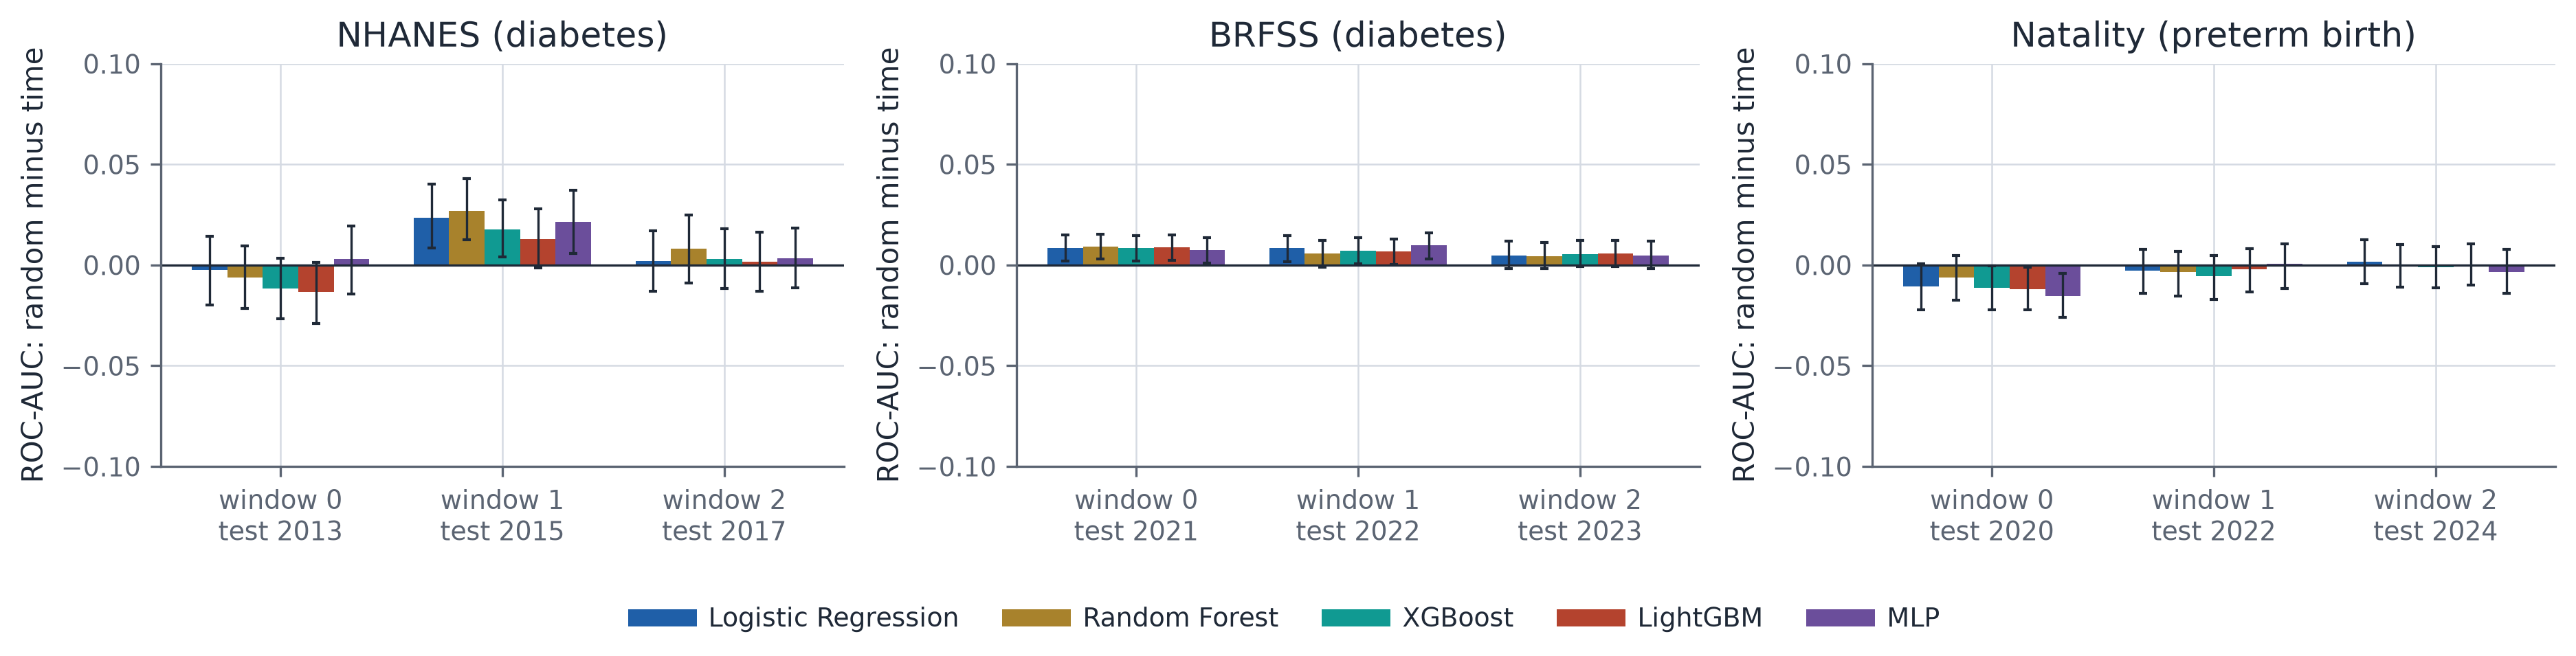
\includegraphics[width=\textwidth]{fig03_random_minus_time.png}
\caption{Random minus time test ROC-AUC per window and model (95\% CI). Positive: random split
overestimates future performance.}
\label{fig:rvt}
\end{figure*}

\begin{table}[!t]
\caption{Random vs.\ time: mean ROC-AUC over windows, gap \eqref{eq:gap}, significant windows, and
rank (time/random).}
\label{tab:rvt}
\centering
\setlength{\tabcolsep}{3.2pt}
\begin{tabular}{@{}llccccc@{}}
\toprule
Data & Model & Time & Random & $\Dgap$ & Sig. & Rank \\
\midrule
\multirow{5}{*}{NHANES} & LightGBM & 0.906 & 0.906 & $+0.000$ & 0 & 1 / 3 \\
 & XGBoost & 0.906 & 0.909 & $+0.003$ & 1 & 2 / 1 \\
 & LR & 0.898 & 0.906 & $+0.008$ & 1 & 3 / 4 \\
 & MLP & 0.897 & 0.906 & $+0.009$ & 1 & \textbf{4 / 2} \\
 & RF & 0.879 & 0.889 & $+0.010$ & 1 & 5 / 5 \\
\midrule
\multirow{5}{*}{BRFSS} & LightGBM & 0.826 & 0.833 & $+0.007$ & 2 & 1 / 1 \\
 & XGBoost & 0.826 & 0.833 & $+0.007$ & 2 & 2 / 2 \\
 & MLP & 0.824 & 0.831 & $+0.007$ & 2 & 3 / 3 \\
 & LR & 0.822 & 0.830 & $+0.007$ & 2 & 4 / 4 \\
 & RF & 0.822 & 0.829 & $+0.006$ & 1 & 5 / 5 \\
\midrule
\multirow{5}{*}{Natality} & XGBoost & 0.753 & 0.747 & $-0.006$ & 1 & 1 / 2 \\
 & LightGBM & 0.753 & 0.749 & $-0.005$ & 1 & 2 / 1 \\
 & MLP & 0.747 & 0.741 & $-0.006$ & 1 & \textbf{3 / 5} \\
 & LR & 0.747 & 0.743 & $-0.004$ & 0 & 4 / 3 \\
 & RF & 0.745 & 0.742 & $-0.003$ & 0 & 5 / 4 \\
\bottomrule
\end{tabular}
\end{table}

\subsection{Same-Period Comparison \contrib{3}}
\label{sec:sameperiod}
Scoring both splits on the same period (Fig.~\ref{fig:same}, Table~\ref{tab:same}):
\begin{itemize}
\item \textbf{Natality:} the gap vanishes (never significant). Later years are easier: XGBoost
scores 0.735 on 2016 rows vs.\ 0.761 on 2020 rows.
\item \textbf{BRFSS:} random stays higher in all 15 model-windows.
\item \textbf{NHANES 2017--18:} the pooled random model is significantly worse ($\approx-0.04$),
plausibly due to the lab-analyzer change (untested).
\end{itemize}

\contribbox{\textbf{\textcolor{contribframe}{Takeaway \contrib{3}.}} Without the same-period
comparison, natality suggests time splits are \emph{easier}; with it, the effect disappears. Temporal
benchmarks should report both.}

\begin{figure*}[!t]
\centering
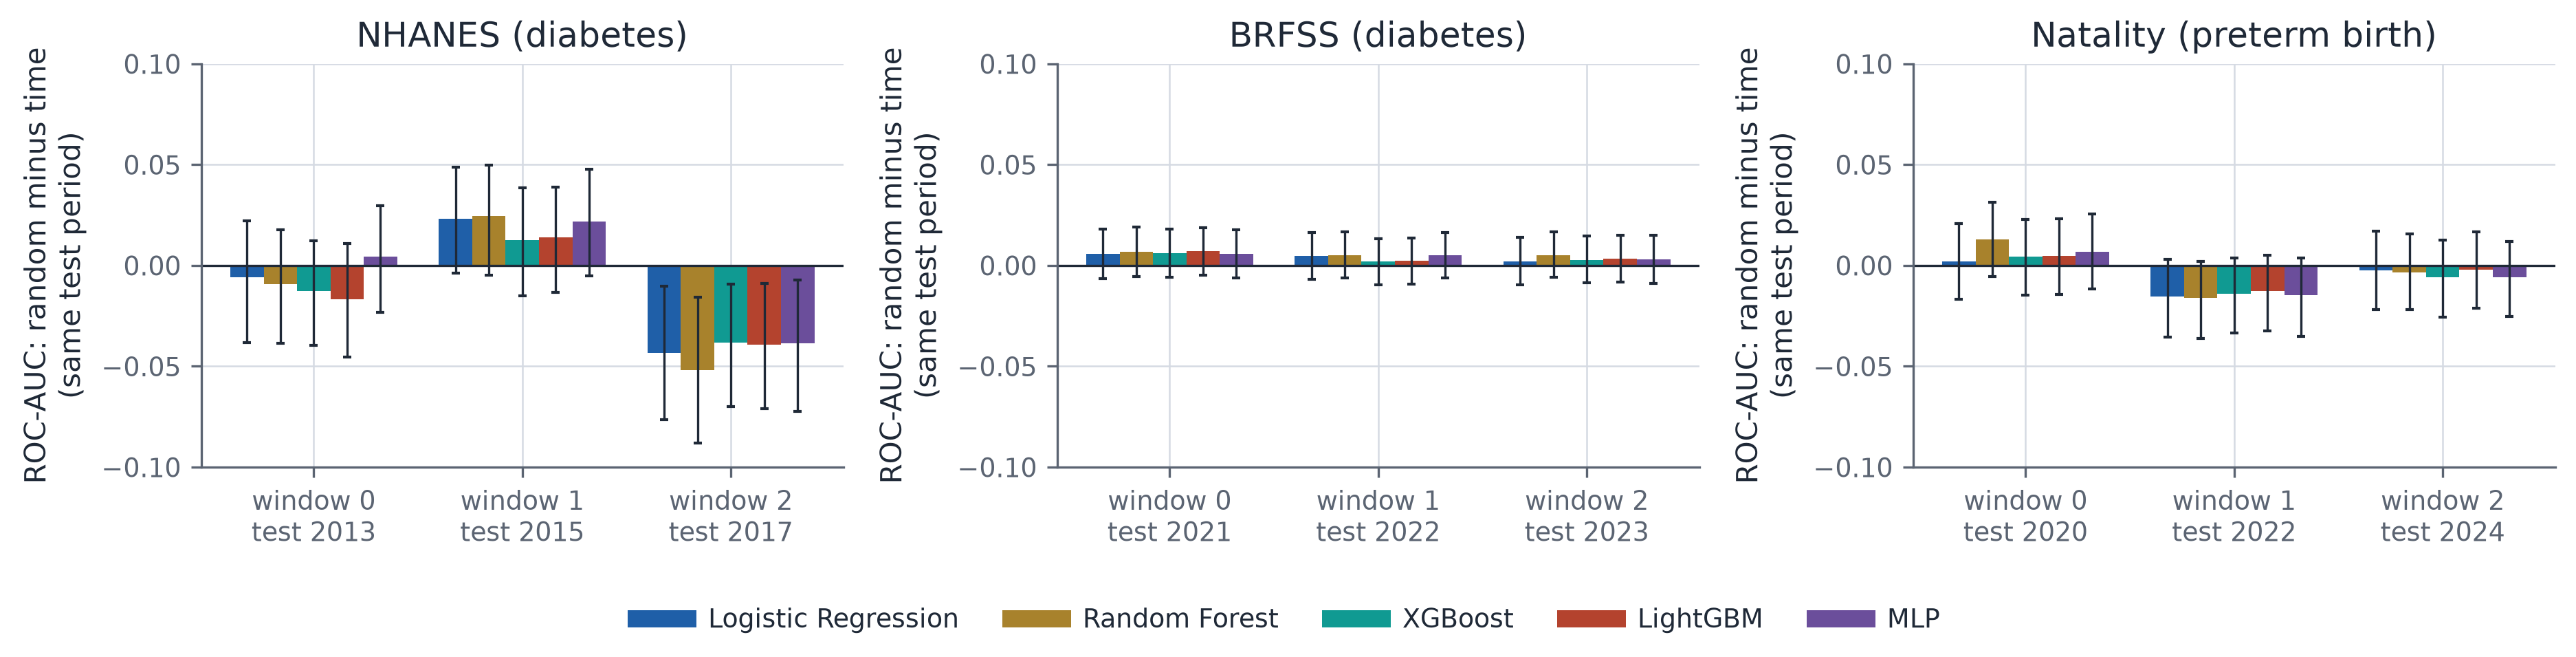
\includegraphics[width=\textwidth]{fig10_random_minus_time_same_period.png}
\caption{Same-period comparison \contrib{3}: random minus time ROC-AUC, both scored on the time
split's test period (95\% CI).}
\label{fig:same}
\end{figure*}

\begin{table}[!t]
\caption{Same-period gap \eqref{eq:samegap}, mean over windows.}
\label{tab:same}
\centering
\setlength{\tabcolsep}{4pt}
\begin{tabular}{@{}llcccc@{}}
\toprule
Data & Model & Time & Random (same) & $\Dgap^{\mathrm{same}}$ & Sig. \\
\midrule
\multirow{5}{*}{NHANES} & LR & 0.898 & 0.889 & $-0.009$ & 1 \\
 & RF & 0.879 & 0.867 & $-0.012$ & 1 \\
 & XGBoost & 0.906 & 0.893 & $-0.013$ & 1 \\
 & LightGBM & 0.906 & 0.892 & $-0.014$ & 1 \\
 & MLP & 0.897 & 0.893 & $-0.004$ & 1 \\
\midrule
\multirow{5}{*}{BRFSS} & LR & 0.822 & 0.827 & $+0.004$ & 0 \\
 & RF & 0.822 & 0.828 & $+0.006$ & 0 \\
 & XGBoost & 0.826 & 0.830 & $+0.004$ & 0 \\
 & LightGBM & 0.826 & 0.831 & $+0.004$ & 0 \\
 & MLP & 0.824 & 0.829 & $+0.005$ & 0 \\
\midrule
\multirow{5}{*}{Natality} & LR & 0.747 & 0.741 & $-0.005$ & 0 \\
 & RF & 0.745 & 0.743 & $-0.002$ & 0 \\
 & XGBoost & 0.753 & 0.748 & $-0.005$ & 0 \\
 & LightGBM & 0.753 & 0.750 & $-0.003$ & 0 \\
 & MLP & 0.747 & 0.742 & $-0.005$ & 0 \\
\bottomrule
\end{tabular}
\end{table}

\subsection{Drift and Its Clinical Causes \contrib{2}}
\label{sec:drift}
NHANES diabetes prevalence rises from 10.4\% to 16.4\% (Fig.~\ref{fig:prev}). Domain-classifier
AUC (Fig.~\ref{fig:domain}) is 0.86--0.97 (NHANES), 0.76--0.79 (BRFSS) and 0.55--0.59 (natality)
for time splits, and $\approx$0.50 for random splits. Table~\ref{tab:events} and
Fig.~\ref{fig:events} list the documented causes. Table~\ref{tab:driftperf} shows that the largest
shift (NHANES 2017--18, domain AUC 0.97) brings no significant gap, while gaps appear with label
shift (NHANES 2015--16) and questionnaire revisions (BRFSS 2021--22): drift type matters more than
size.

\begin{figure*}[!t]
\centering
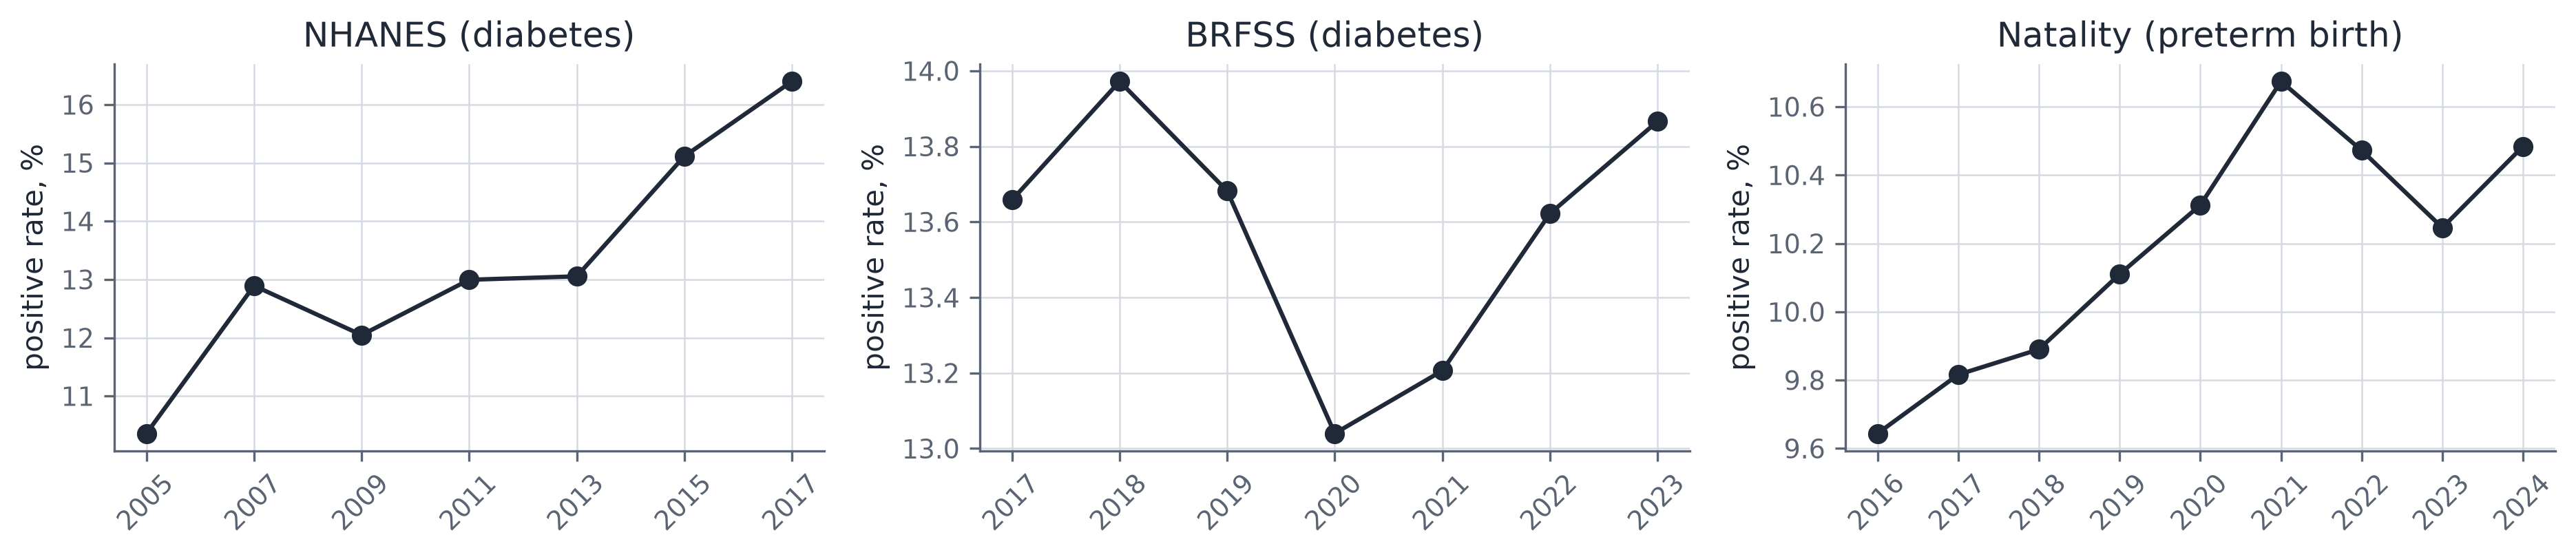
\includegraphics[width=\textwidth]{fig01_prevalence.png}
\caption{Label shift: positive rate per period.}
\label{fig:prev}
\end{figure*}

\begin{figure*}[!t]
\centering
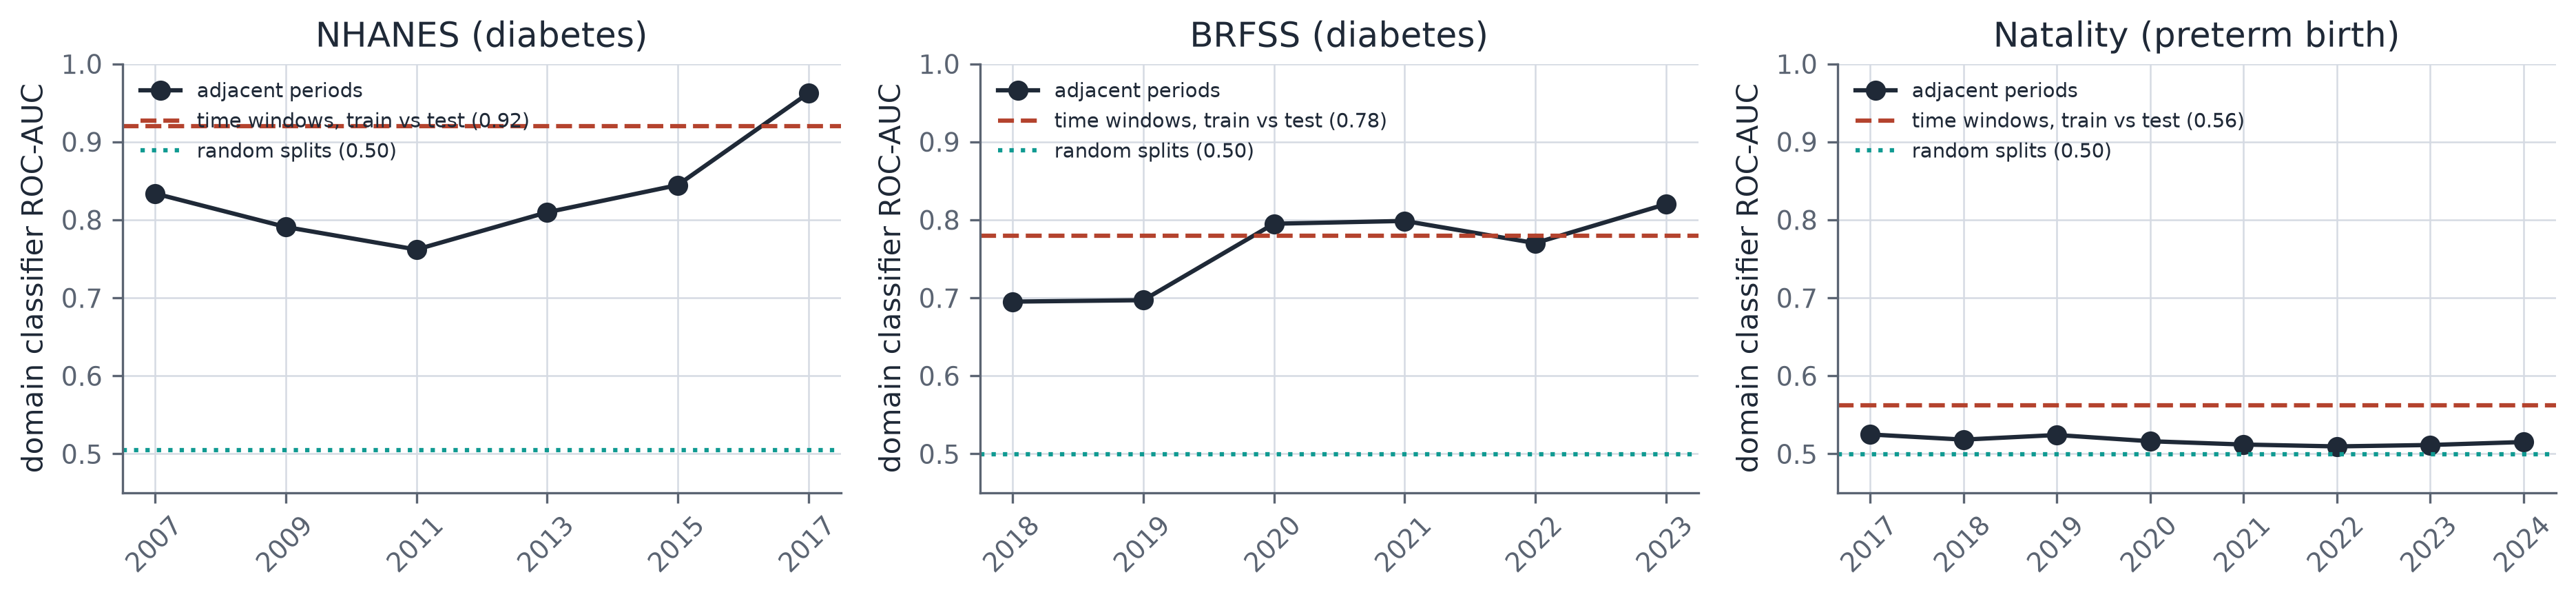
\includegraphics[width=\textwidth]{fig07_domain_shift.png}
\caption{Covariate shift: domain-classifier ROC-AUC between periods (0.5 = no shift).}
\label{fig:domain}
\end{figure*}

\begin{table*}[!t]
\caption{Drift with a documented clinical cause \contrib{2}, measured in our tables.}
\label{tab:events}
\centering
\resizebox{\textwidth}{!}{%
\begin{tabular}{@{}lllll@{}}
\toprule
Dataset & Change & Period & Measured size & Cause type \\
\midrule
\multirow{4}{*}{NHANES} & Hematology analyzer replaced (Beckman Coulter DxH 800) & 2013--14 & mean RDW 13.07 $\rightarrow$ 13.73 (CDC: 12.84\% $\rightarrow$ 13.55\%) & lab instrument \\
 & Biochemistry analyzer and lab changed (Roche Cobas 6000) & 2017--18 & LDH 129 $\rightarrow$ 159; AST 25.9 $\rightarrow$ 22.0 & lab instrument \\
 & Affordable Care Act (2014) & 2015--18 & uninsured 25.6\% (2009--10) $\rightarrow$ 15.2\%; Medicaid 8.1\% $\rightarrow$ 17.6\% & policy \\
 & Diagnosed diabetes rising & all & 10.4\% $\rightarrow$ 16.4\% & label \\
\midrule
\multirow{4}{*}{BRFSS} & Personal-doctor question reworded & 2021 & ``more than one'' 6.7\% $\rightarrow$ 28.4\% & coding revision \\
 & Coverage question replaced & 2021 & no coverage 8.6\% $\rightarrow$ 5.2\% & coding revision \\
 & Race category ``other race only'' removed & 2022 & 3.0\% $\rightarrow$ 0\% & coding revision \\
 & Shift to cell-phone sample & all & landline item missing 57\% $\rightarrow$ 81\% & survey mode \\
\midrule
\multirow{4}{*}{Natality} & California withholds marital status & 2017 & missing 0\% $\rightarrow$ 12\% & reporting law \\
 & Gestational hypertension & all & 5.9\% $\rightarrow$ 10.3\% & population / practice \\
 & Smoking before pregnancy & all & 1.23 $\rightarrow$ 0.39 cigarettes/day & population \\
 & COVID-19 hospital policies (father info) & 2020 & missing 11.6\% $\rightarrow$ 12.6\% & protocol \\
\bottomrule
\end{tabular}}
\end{table*}

\begin{figure*}[!t]
\centering
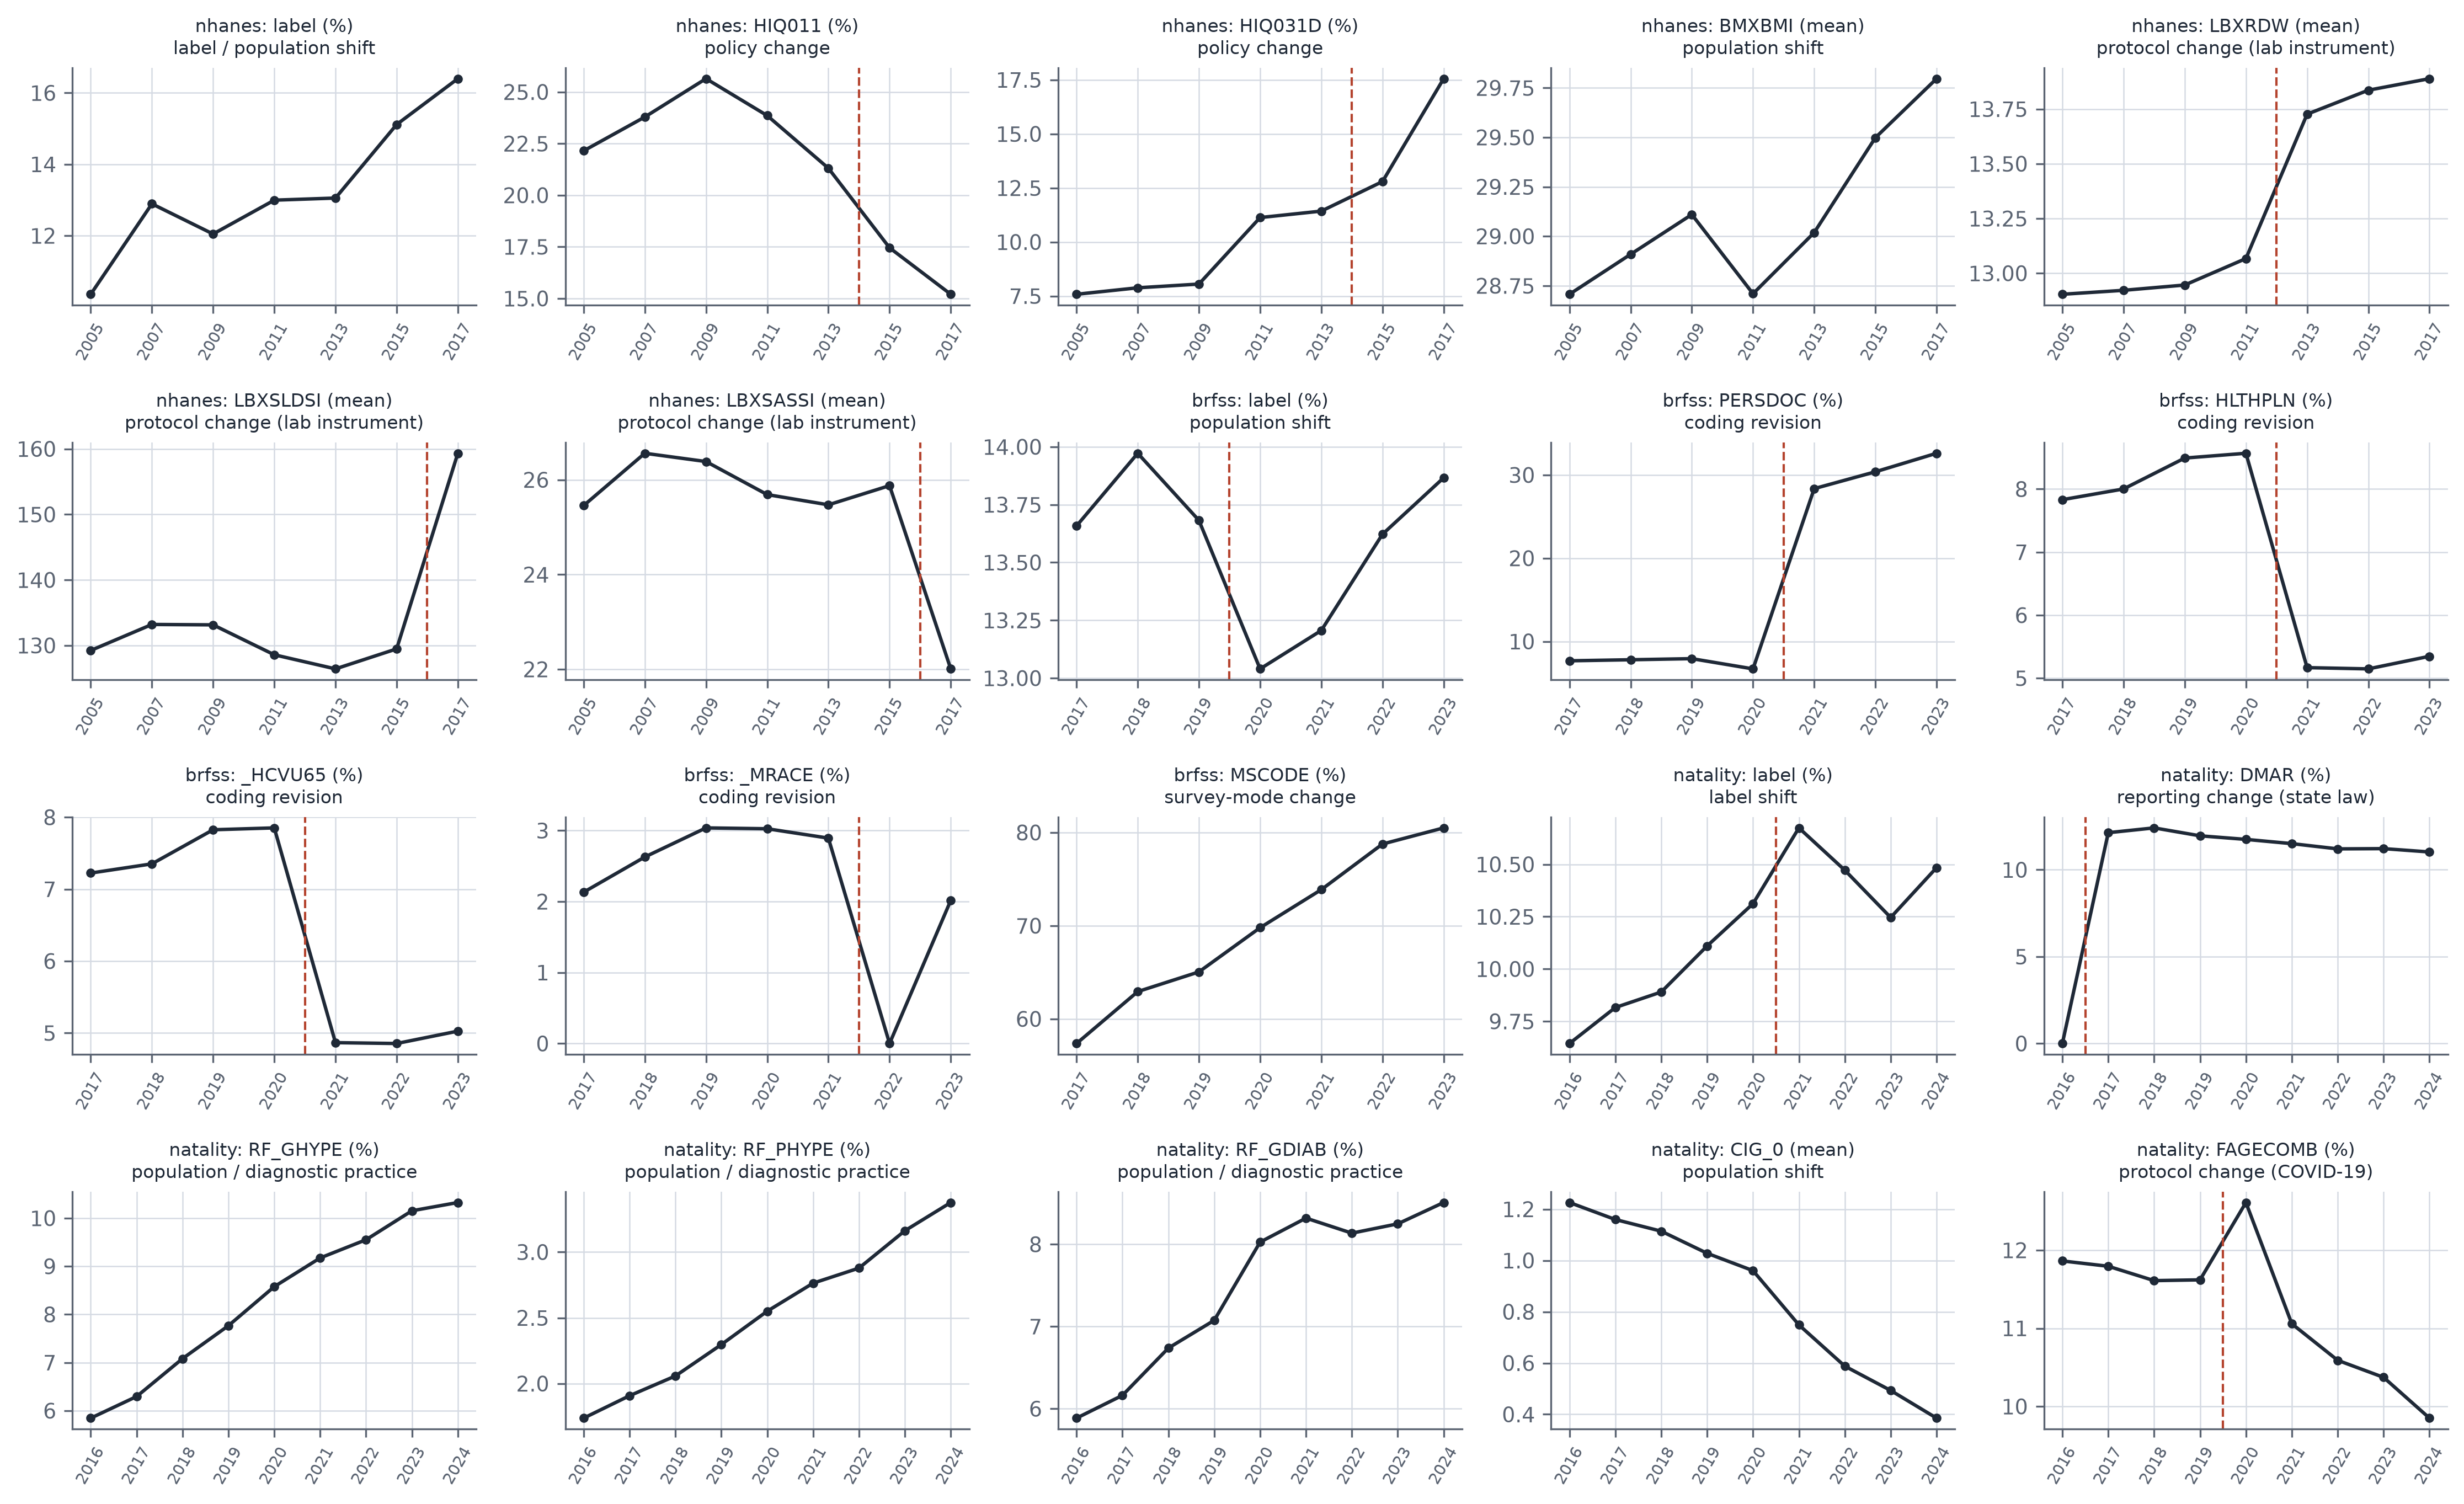
\includegraphics[width=0.88\textwidth]{fig08_drift_events.png}
\caption{Documented drift events per period \contrib{2} (dashed line: period of the change).}
\label{fig:events}
\end{figure*}

\begin{table*}[!t]
\caption{Drift vs.\ performance per sliding window.}
\label{tab:driftperf}
\centering
\resizebox{\textwidth}{!}{%
\begin{tabular}{@{}llcccccl@{}}
\toprule
Dataset & Window (test) & Domain AUC & Prev.\ train & Prev.\ test & $\Dgap$ (mean) & Sig.\ models & Events in test period \\
\midrule
\multirow{3}{*}{NHANES} & 0 (2013--14) & 0.864 & 0.119 & 0.131 & $-0.006$ & 0 & hematology analyzer \\
 & 1 (2015--16) & 0.921 & 0.126 & 0.151 & $+0.020$ & 4 & prevalence jump; ACA \\
 & 2 (2017--18) & \textbf{0.974} & 0.127 & 0.164 & $+0.004$ & 0 & biochemistry analyzer \\
\midrule
\multirow{3}{*}{BRFSS} & 0 (2021) & 0.790 & 0.138 & 0.132 & $+0.008$ & 5 & doctor / insurance questions \\
 & 1 (2022) & 0.784 & 0.136 & 0.136 & $+0.008$ & 4 & race question \\
 & 2 (2023) & 0.766 & 0.133 & 0.139 & $+0.005$ & 0 & none \\
\midrule
\multirow{3}{*}{Natality} & 0 (2020) & 0.570 & 0.098 & 0.103 & $-0.011$ & 3 & COVID-19 year \\
 & 1 (2022) & 0.564 & 0.101 & 0.105 & $-0.003$ & 0 & none \\
 & 2 (2024) & 0.552 & 0.105 & 0.105 & $-0.000$ & 0 & none \\
\bottomrule
\end{tabular}}
\end{table*}

\subsection{Comparison with State of the Art \contrib{4}}
\label{sec:sota}
GBDTs and the MLP are TabReD's reference baselines \cite{rubachev2025tabred,grinsztajn2022why}.
In TabReD, XGBoost's lead over the MLP shrinks under time splits ($+2.02\%\rightarrow+0.91\%$); on
clinical data it grows in NHANES ($+0.28\%\rightarrow+0.97\%$) and is unchanged elsewhere
(Table~\ref{tab:sota}). Random splits \emph{hide} the GBDT advantage here. TableShift's BRFSS
accuracies (0.877/0.832) \cite{gardner2023tableshift} use a group shift and a different threshold,
so they are not directly comparable.

\begin{table}[!t]
\caption{\% ROC-AUC improvement over the MLP \eqref{eq:improve}. TabReD: its Table 4.}
\label{tab:sota}
\centering
\setlength{\tabcolsep}{3.5pt}
\begin{tabular}{@{}llcccc@{}}
\toprule
Benchmark & Splits & LR & RF & XGBoost & LightGBM \\
\midrule
\multirow{2}{*}{TabReD \cite{rubachev2025tabred}} & time & -- & -- & $+0.91$ & -- \\
 & random & -- & -- & $+2.02$ & -- \\
\midrule
\multirow{2}{*}{NHANES} & time & $+0.09$ & $-2.00$ & $\mathbf{+0.97}$ & $\mathbf{+0.99}$ \\
 & random & $-0.08$ & $-1.94$ & $+0.28$ & $-0.00$ \\
\multirow{2}{*}{BRFSS} & time & $-0.20$ & $-0.23$ & $+0.24$ & $+0.28$ \\
 & random & $-0.22$ & $-0.35$ & $+0.19$ & $+0.24$ \\
\multirow{2}{*}{Natality} & time & $-0.07$ & $-0.22$ & $+0.84$ & $+0.83$ \\
 & random & $+0.23$ & $+0.15$ & $+0.85$ & $+1.03$ \\
\bottomrule
\end{tabular}
\end{table}

% =====================================================================================
\section{Discussion}
\label{sec:discussion}
Table~\ref{tab:claims} answers the research questions. \textbf{RQ1:} random splits overestimate
where labels shift or questionnaires change and reorder models in NHANES. \textbf{RQ2:} GBDTs
transfer best; validating on a single later period can still pick the wrong model. \textbf{RQ3:}
large shifts have documented causes (instruments, wording, policy, reporting rules).
\textbf{RQ4:} drift type, not size, predicts the gap, so a domain-classifier AUC alone is a weak
warning signal.

\begin{table*}[!t]
\caption{TabReD's claims on clinical data \contrib{4}.}
\label{tab:claims}
\centering
\begin{tabular}{@{}p{5.0cm}p{3.7cm}p{3.9cm}p{3.6cm}@{}}
\toprule
TabReD claim & NHANES (280 features) & BRFSS (93) & Natality (73) \\
\midrule
Random splits overestimate future performance & yes, label-shift window & yes, small, coding-revision years & no (period-difficulty artefact) \\
Random splits change the model ranking & yes (MLP 2nd $\rightarrow$ 4th) & no & partly (MLP, LR) \\
GBDTs are the strongest models & yes & yes & yes \\
XGBoost's lead over MLP shrinks under time splits & no, it grows & no & no \\
\bottomrule
\end{tabular}
\end{table*}

\textbf{Limitations:} one seed and small grids; no CatBoost \cite{prokhorenkova2018catboost},
MLP-PLR or FT-Transformer; a plain scikit-learn MLP; small same-period samples in NHANES; causal
explanations are hypotheses; no survey weights.

% =====================================================================================
\section{Conclusion and Future Work}
\label{sec:conclusion}
Clinical TabReD shows that GBDTs remain best on clinical data, that random splits overestimate and
reorder models where labels shift or questionnaires change but not for preterm birth, and that
XGBoost's lead over the MLP grows under time splits. Our same-period comparison \contrib{3} reveals
that part of the random-vs-time signal is period difficulty. Future work: more seeds and Optuna
tuning, MLP-PLR/FT-Transformer/CatBoost, shift-robust training and recalibration
\cite{lipton2018detecting}, and EHR data with real deployment times.

\section*{Acknowledgment}
We thank Dr.~Hari Mohan Rai for guidance. Data are public CDC/NCHS files.

\bibliographystyle{IEEEtran}
\bibliography{references}

\end{document}
